\documentclass[%
 reprint,
 superscriptaddress,
 amsmath,
 amssymb,
 prstab,
]{revtex4-1}

\usepackage{graphicx}% Include figure files
\usepackage{dcolumn}% Align table columns on decimal point
\usepackage{bm}% bold math
\usepackage{subcaption}

\begin{document}
\maxdeadcycles=1000

\title{Design, Commissioning and Operation of the CTF3 Phase Feedforward System}

\author{J.~Roberts}
\email{Corresponding author Jack.Roberts@cern.ch}
\affiliation{John Adams Institute (JAI), University of Oxford, Denys Wilkinson 
Building, Keble Road, Oxford, OX1 3RH, United Kingdom}
\affiliation{The European Organization for Nuclear Research (CERN), Geneva 23, 
CH-1211, Switzerland}

\author{P.~Skowronski}
\affiliation{The European Organization for Nuclear Research (CERN), Geneva 23, 
	CH-1211, Switzerland}

\author{P.~Burrows}
\affiliation{John Adams Institute (JAI), University of Oxford, Denys Wilkinson 
Building, Keble Road, Oxford, OX1 3RH, United Kingdom}

\author{G.~Christian}
\affiliation{John Adams Institute (JAI), University of Oxford, Denys Wilkinson 
Building, Keble Road, Oxford, OX1 3RH, United Kingdom}

\author{R.~Corsini}
\affiliation{The European Organization for Nuclear Research (CERN), Geneva 23, 
CH-1211, Switzerland}

\author{A.~Ghigo}
\affiliation{Laboratori Nazionali di Frascati (LNFN), Via Enrico Fermi, 40, 
00044 
Frascati RM, Italy}

\author{F.~Marcellini}
\affiliation{Laboratori Nazionali di Frascati (LNFN), Via Enrico Fermi, 40, 
00044 
Frascati RM, Italy}

\author{C.~Perry}
\affiliation{John Adams Institute (JAI), University of Oxford, Denys Wilkinson 
Building, Keble Road, Oxford, OX1 3RH, United Kingdom}


\date{\today}

\begin{abstract}
Abstract
\end{abstract}

\maketitle

\section{\label{sec:intro}Introduction}

%PRL
A major challenge is the synchronisation of the arrival of the drive and main 
beams at the power-extraction and transfer structures to better than 50~fs rms. 
This requirement limits the luminosity loss, resulting from subsequent 
energy errors of the main beams, to less than 1\% of the design 
value~\cite{clicLumEq}.
In the CLIC design the incoming drive-beam phase jitter 
cannot be guaranteed to be better than \(2^\circ\)~\cite{CLICCDR}.
A mechanism 
to improve the phase stability by an order of magnitude is 
therefore required. The correction must be applied to the full drive beam pulse 
length and have a bandwidth exceeding 17.5~MHz~\cite{Gerber2015}. 

This is implemented via a `phase feed-forward' (PFF) system which measures the 
incoming beam phase and provides a correction to the same beam pulse 
after it has traversed the turnaround loop (TA in Fig.~\ref{fig:CLICLayout}). 
The incoming beam phase is measured in two upstream phase 
monitors (\(\phi_{1}, \phi_{2}\)). While the beam 
transits the ‘turnaround loop’ a phase-correction signal is evaluated and used 
to drive fast, high power amplifiers; these drive two electromagnetic kickers 
(\(\mathrm{K_1, K_2}\)) which are used to alter the beam transit time in a 
four-bend chicane. A downstream phase monitor (\(\phi_{3}\)) is 
used to measure the effect of the correction. 

The beam time of flight between \(\phi_1\) and \(\mathrm{K_1}\) is around 
380~ns. The total cable delay for the PFF correction signals 
is shorter, around 250~ns. The correction in the chicane can therefore be 
applied to the entirety of the beam pulse measured at the PFF input 
(\(\phi_1\)), provided that the hardware latency is less than 130~ns. 
Significant hardware challenges include the resolution and bandwidth of the 
phase monitors, and the power, latency and bandwidth of the kicker amplifiers. 
A low latency digitiser/feedforward controller is also required.
%/PRL

Key results from the CTF3 PFF system have previously been published in [REF]. 
This paper presents a more detailed description of the design and commissioning 
of the system - the hardware, the optics, the correction timing, and additional 
results.

CLIC intro/PFF system.

CTF3 layout, parameters etc.

CTF PFF system.

\begin{figure}
	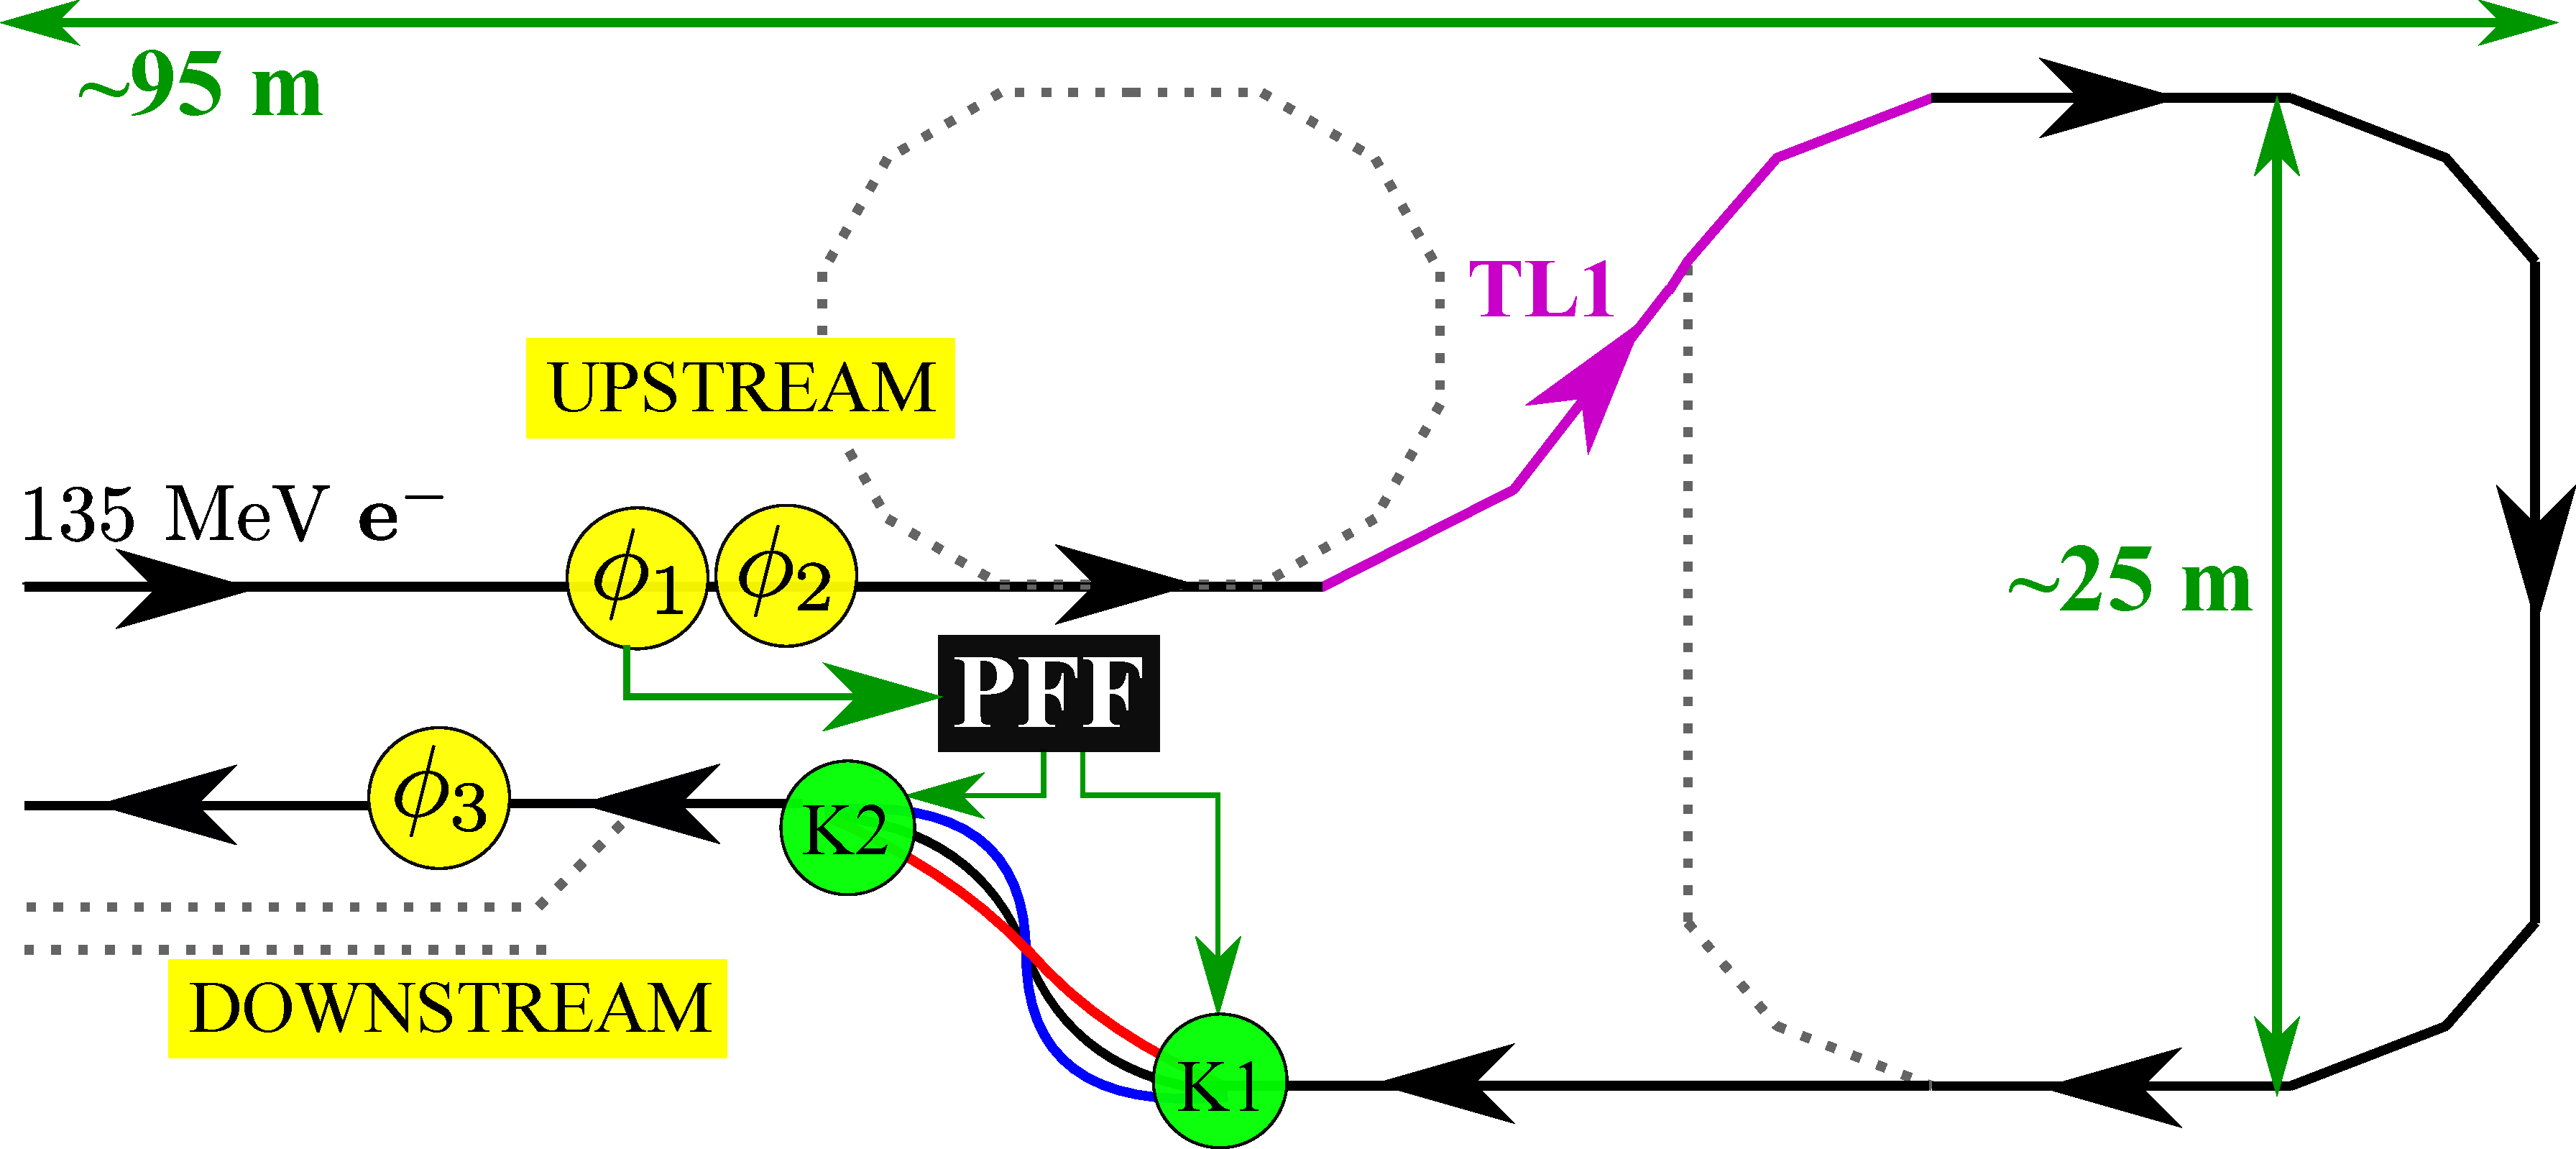
\includegraphics[width=\columnwidth]{figs/intro/ctfpffLayout}% Here is 
	%how to 
	%import EPS art
	\caption{\label{f:pffLayout}Schematic of the PFF prototype at CTF3, 
	showing the phase monitors (\(\phi_1\) , 
	\(\phi_2\) and \(\phi_3\)) and kickers (K1 and K2). The black box “PFF” 
	represents the calculation and output of the correction, including the 
	phase monitor electronics, feedforward controller and kicker amplifiers.
	Dashed lines indicate beam lines that are not used during PFF operation. 
	Bunches arriving early at the upstream monitor (\(\phi_1\)) are directed 
	on to longer trajectories in the correction chicane (blue), and bunches 
	arriving late on to shorter trajectories (red).
		}
\end{figure}

\section{\label{s:hw}Hardware}

\subsection{\label{ss:phMon}Phase Monitors}

\begin{figure}
	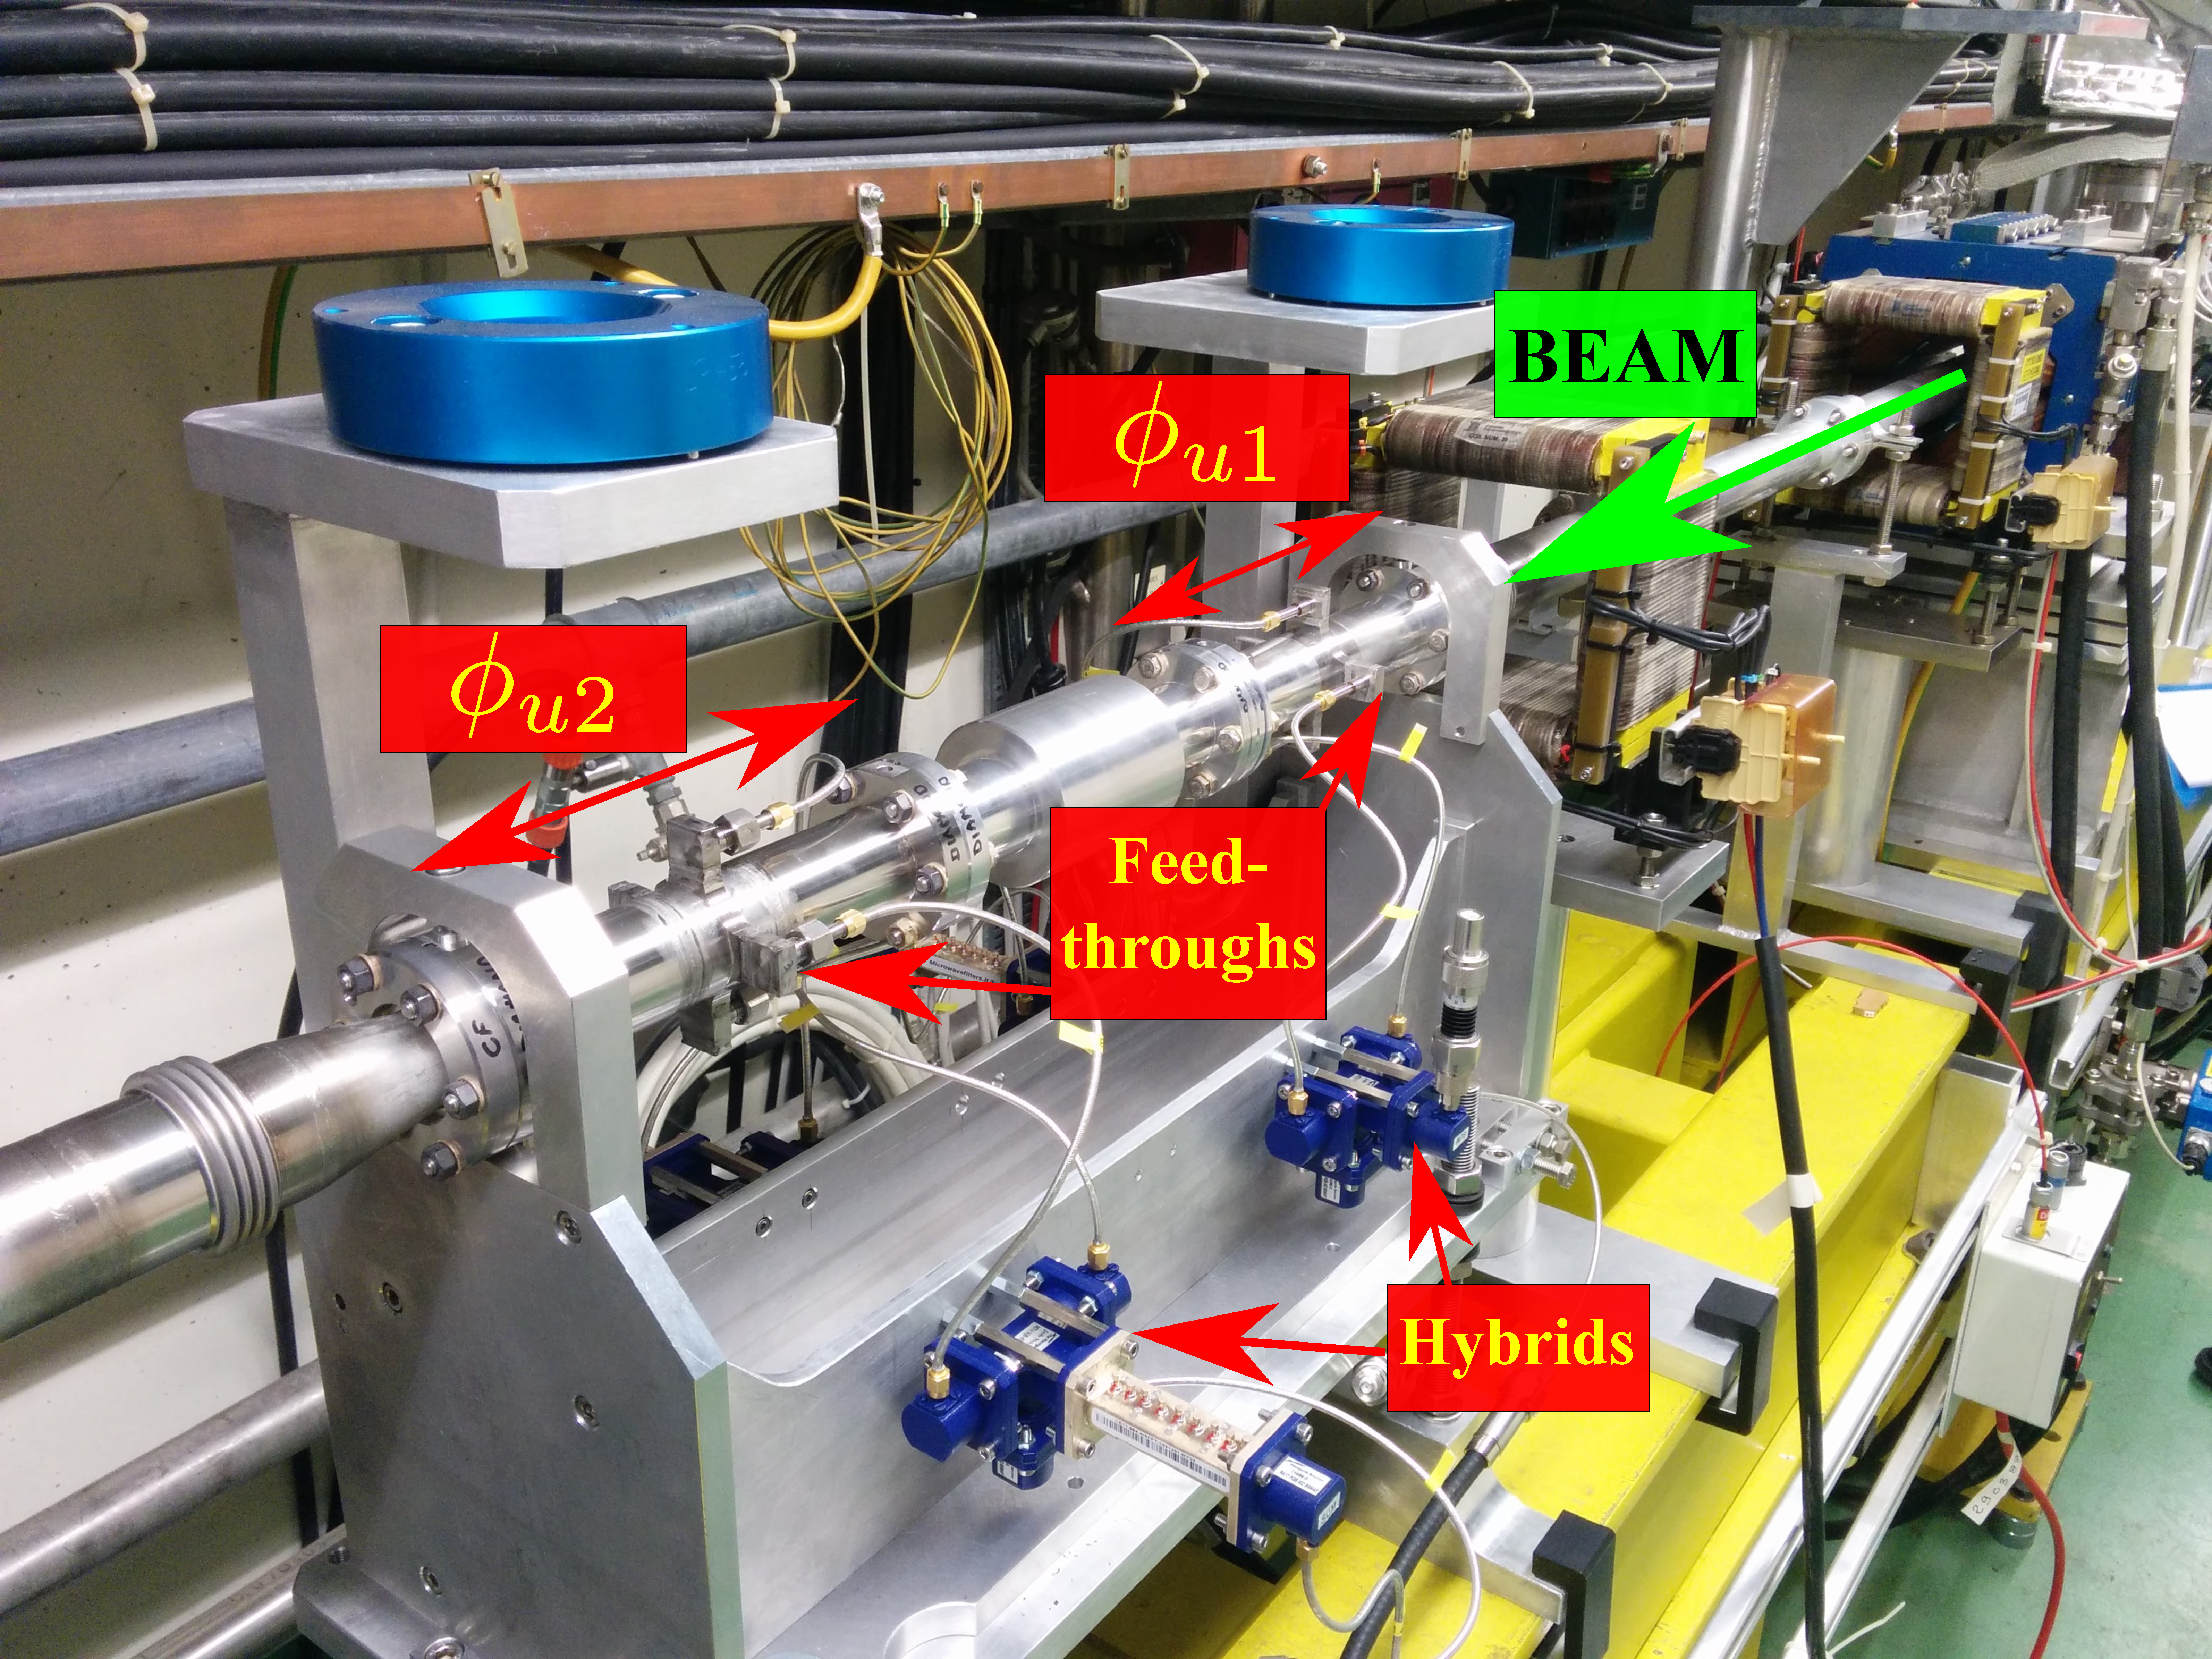
\includegraphics[width=\columnwidth]{figs/hw/phMonCTPic}
	\caption{\label{f:phMonCTPic}The installation of the upstream phase 
		monitors (\(\phi_{u1}\) and \(\phi_{u2}\)) in the beam line.}
\end{figure}

Three phase monitors were installed at CTF3 for the PFF prototype -- two 
neighbouring monitors upstream, \(\phi_{u1}\) and \(\phi_{u2}\), and one 
downstream of the correction chicane, \(\phi_{d}\). Fig.~\ref{f:phMonCTPic} 
shows the installation of the upstream phase monitors 
in the beam line. The upstream monitors are 
used to provide the PFF input (typically \(\phi_{u1}\)), and to measure the 
phase monitor resolution. The notation \(\phi_u\) 
will be used where the distinction between the measurements at \(\phi_{u1}\) 
and \(\phi_{u2}\) is unimportant. The downstream monitor, \(\phi_{d}\), is used 
to measure the effect of the PFF correction.

The phase monitors are cylindrical cavities with an external device length of 
approximately 19~cm and an internal diameter of 23~mm. Small ridges (notch 
filters) in the cavity create 
a volume resonating at 12~GHz (the CLIC drive beam frequency) which contains 
the beam induced fields and reflects any stray 12~GHz fields. The signals are 
extracted through horizontal and vertical pairs of rectangular waveguides, 
before transitioning to 50~\(\mathrm{\Omega}\) coaxial cable via RF 
feedthroughs \cite{phMonIPAC10}. The cavities support the TM01 monopole and 
TE11 dipole modes. The position dependent dipole mode is removed by summing the 
pair of vertical outputs in 180 degree hybrids. The horizontal pair is 
instrumented in the same way but typically is not used. 

\begin{figure}
	\includegraphics[width=\columnwidth]{figs/hw/racks}% Here is 
	%how to 
	%import EPS art
	\caption{\label{f:racks}The two racks containing the PFF system hardware -- 
		the phase monitor electronics, feedforward controller and the kicker 
		amplifiers.}
\end{figure}

The electronics used to extract the phase measurement from the cavity signals 
are installed on the floor above the machine hall in the CTF3 ``klystron 
gallery'', alongside the other hardware used for the PFF system 
(Fig.~\ref{f:racks}). 
Each set of electronics produces two outputs - a phase 
dependent ``mixer'' signal, and a power dependent ``diode'' signal. 

The beam induced signal from the cavities is down-mixed with a 12~GHz local 
oscillator (LO) to create the mixer output. The LO is generated 
from a common 3~GHz source that is phase-locked to the CTF3 drive beam.
Each set of electronics has dedicated frequency multipliers, to increase the LO 
frequency to 12~GHz, and phase shifters, used for calibrations (see below). To 
be able to operate the mixers at low power (to improve linearity) whilst 
maintaining a large signal to noise ratio (to improve resolution) eight 
separate mixers and diodes are used in each set of 
electronics \cite{alex09}. The inputs are split between the eight 
mixers and diodes, with the final two outputs being the sum of the individual 
mixer and diode signals. 
Fig.~\ref{f:phMonDiagram} shows a simplified example of this with two 
mixers and diodes. 

\begin{figure}
	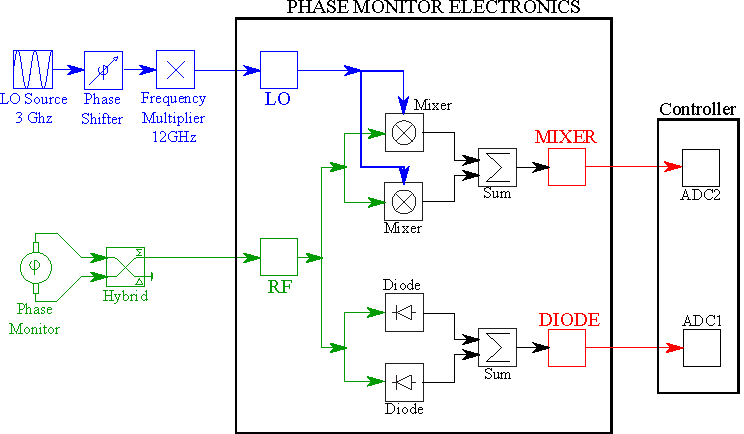
\includegraphics[width=\columnwidth]{figs/hw/phMonDiagram}% Here is 
	%how to 
	%import EPS art
	\caption{\label{f:phMonDiagram}
	}
\end{figure}

The diode output was intended to be used to power normalise the mixer output. 
However, an unforeseen design issue with the electronics resulted in the diodes 
saturating at a much lower input voltage than the mixers 
(Fig.~\ref{f:MixDioVsVolts}). To be able to achieve the best possible 
resolution from the mixers, the electronics were operated with the diodes 
saturated, and the diode outputs were not used in the phase reconstruction as 
envisaged. As a consequence, calibrations had to be repeated regularly to 
account for any differences in output power from the cavities resulting from 
changes to the beam setup.

\begin{figure}
	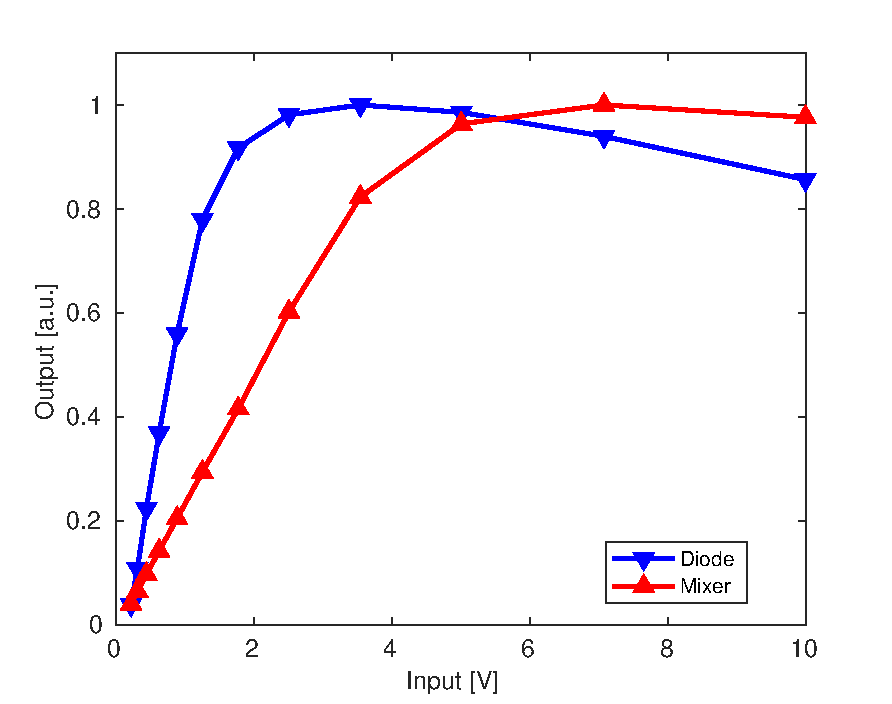
\includegraphics[width=\columnwidth]{figs/hw/MixDioVsVolts}
	\caption{\label{f:MixDioVsVolts}Electronics diode and mixer output 
	amplitudes (normalised with respect to their peak output) versus the input 
	voltage.}
\end{figure}

% FROM THESIS
The phase, \(\phi(t)\), was therefore calculated from the ``Mixer'' outputs as 
follows:
\begin{align}
	&\mathrm{Mixer}(t) = A\sin[\phi(t)] + d \\
	&\phi(t) = \arcsin\left(\frac{\mathrm{Mixer}(t)-d}{A}\right)
	\label{e:phaseRecUsed}
\end{align}
Two calibration constants are needed -- \(A\) and \(d\). \(A\) is the fitted 
(power dependent) 
amplitude of the sinusoidal mixer output, and \(d\) is the asymmetry or offset 
between the maximum and minimum mixer output.
% /FROM THESIS

Point by point and mean resolution

Bandwidth

Position dependence

% FROM THESIS
Figure~\ref{f:horizontalPosScan} shows the results of a horizontal position 
scan in the upstream phase monitors, with the phase plotted against the 
horizontal position in the BPM.

Taking the calculated position dependence of Mon~1 and Mon~2 this corresponds 
to only an additional measured phase jitter of roughly \(0.04^\circ\), using 
the larger dependence in the horizontal plane. This is small compared to the 
phase monitor resolution
% /FROM THESIS

%\begin{figure}
%	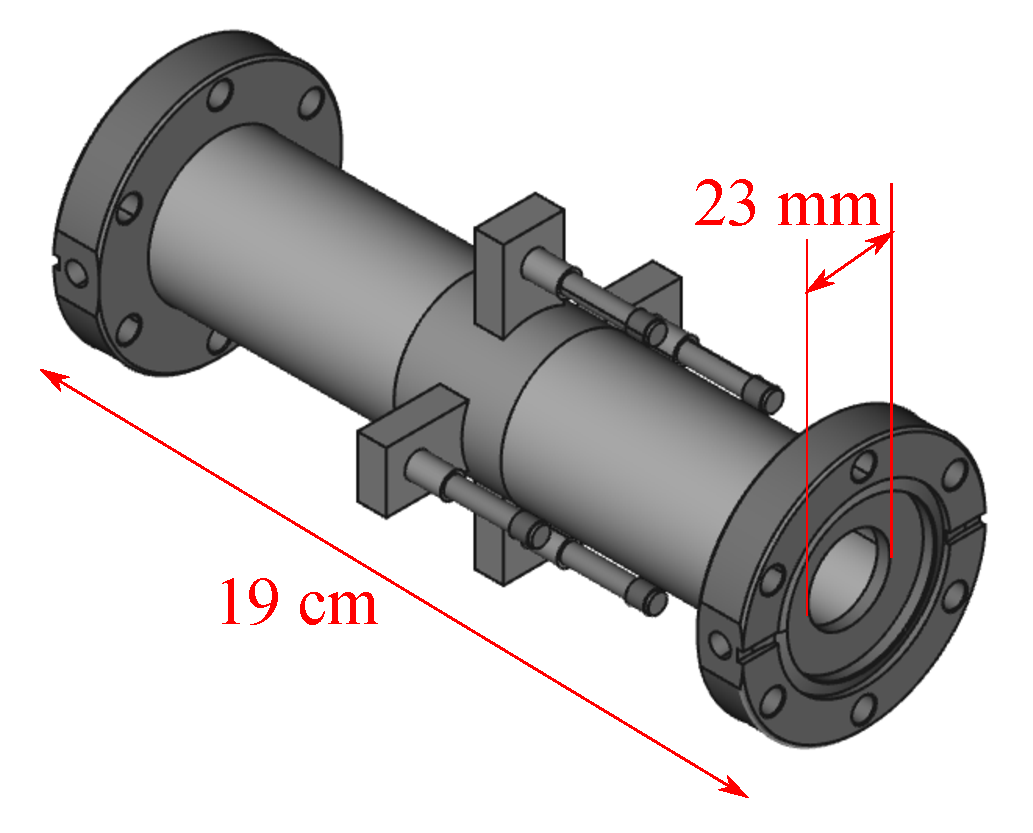
\includegraphics[width=\columnwidth]{figs/hw/phMonTechDraw}% Here is 
%	%how to 
%	%import EPS art
%	\caption{\label{f:phMonTechDraw}
%	}
%\end{figure}
%\begin{figure}
%	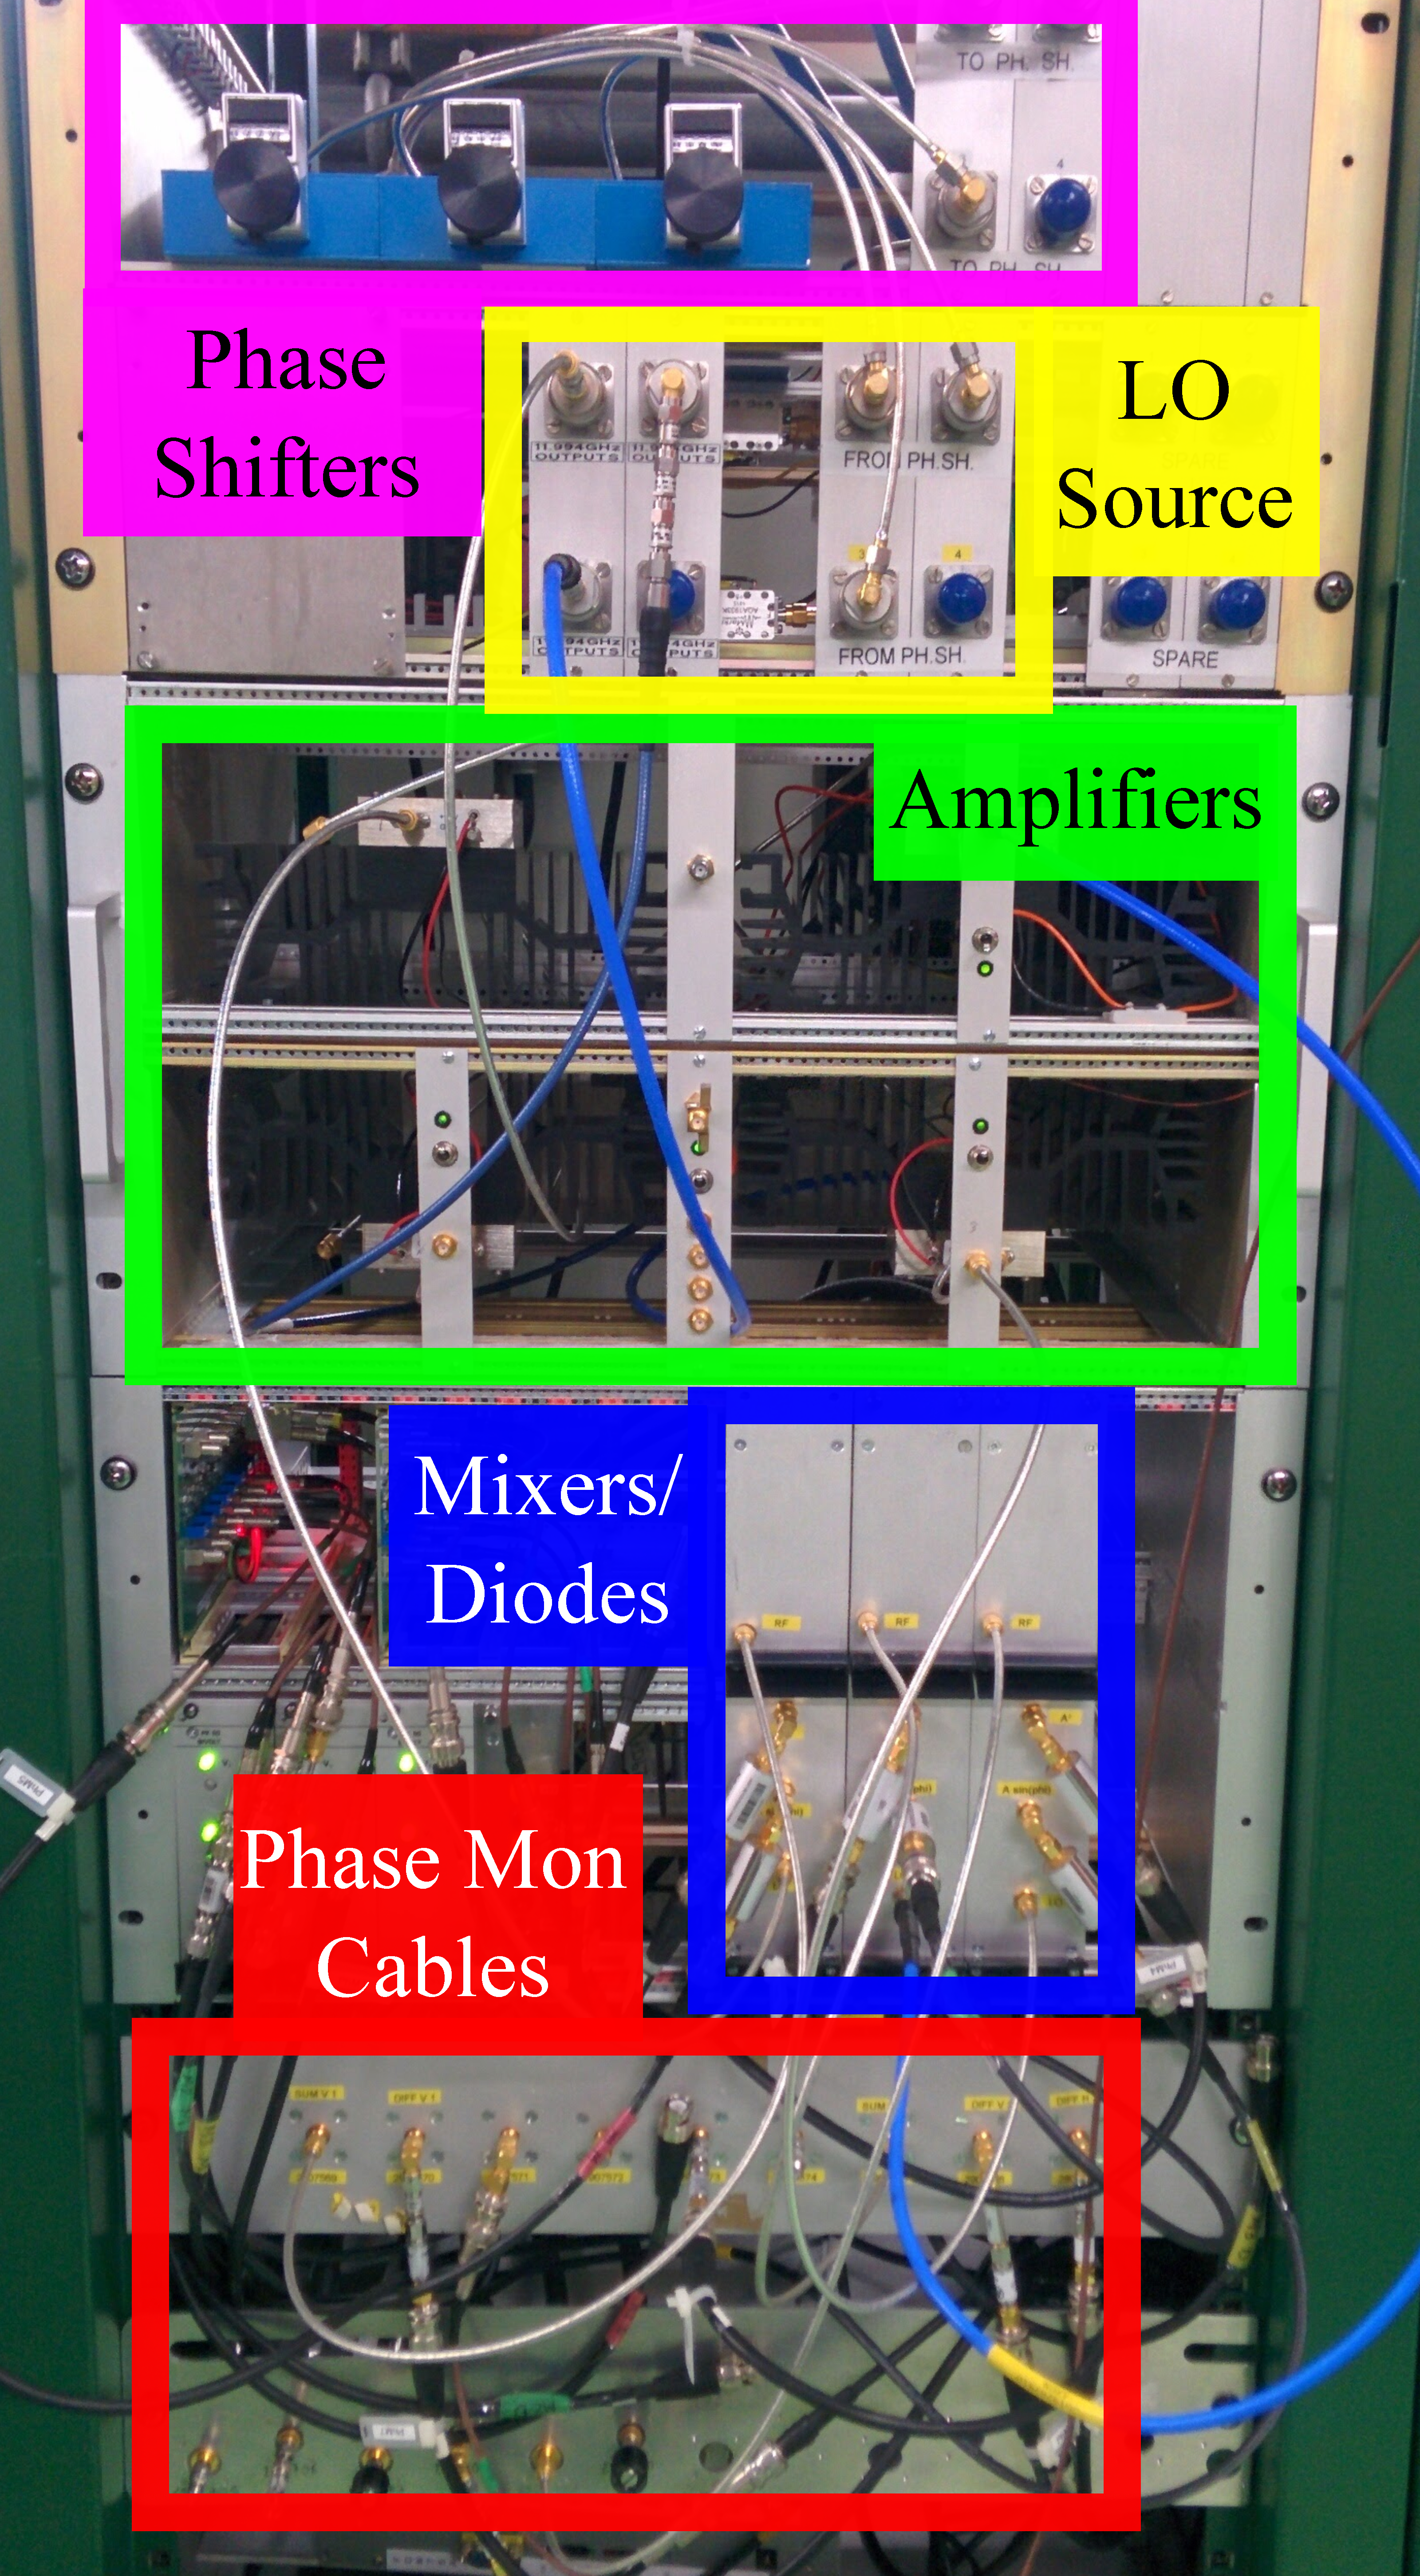
\includegraphics[width=\columnwidth]{figs/hw/phMonRack}% Here is 
%	%how to 
%	%import EPS art
%	\caption{\label{f:phMonRack}
%	}
%\end{figure}

\begin{figure}
	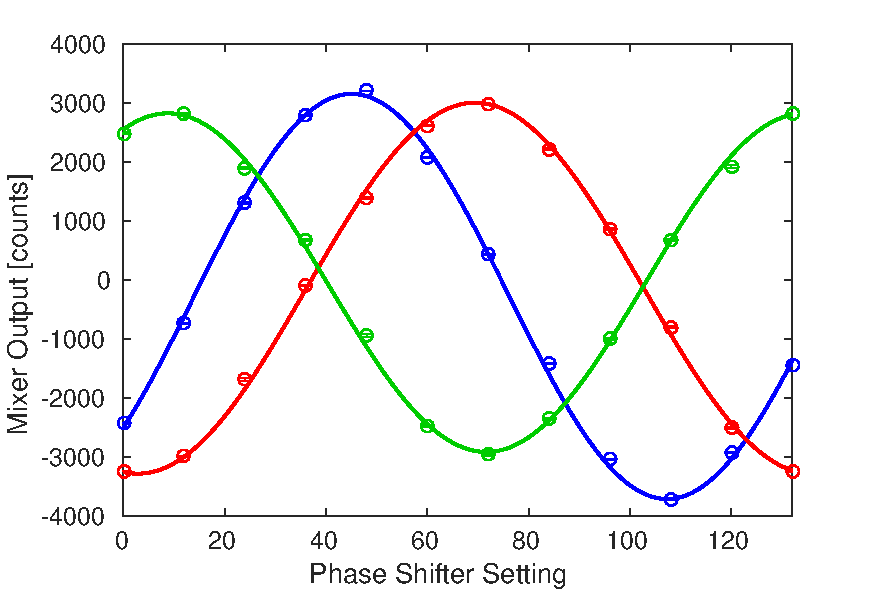
\includegraphics[width=\columnwidth]{figs/hw/phMonCal}% Here is 
	%how to 
	%import EPS art
	\caption{\label{f:phMonCal}
	}
\end{figure}

\begin{figure}
	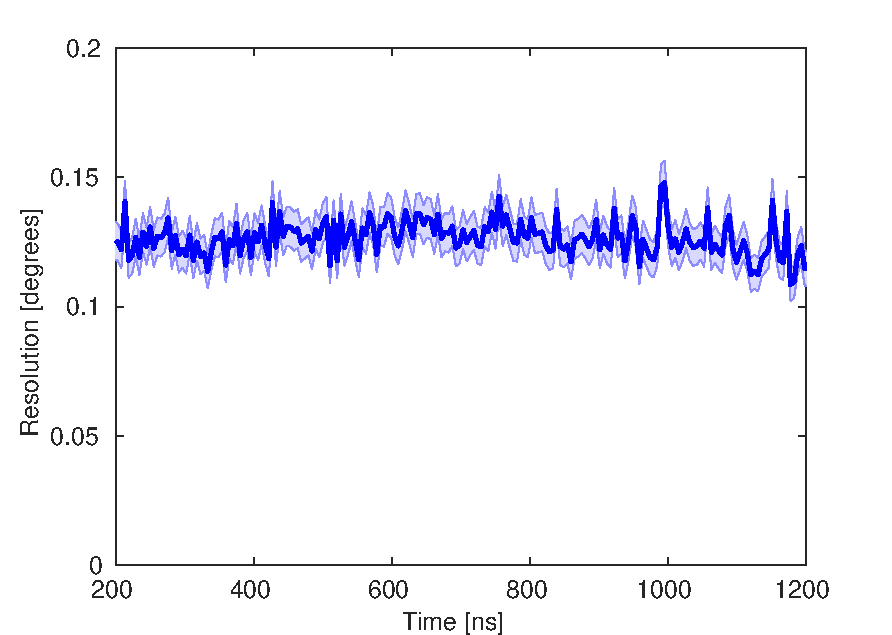
\includegraphics[width=\columnwidth]{figs/hw/phMonRes}% Here is 
	%how to 
	%import EPS art
	\caption{\label{f:phMonRes}
	}
\end{figure}

%\begin{figure}
%	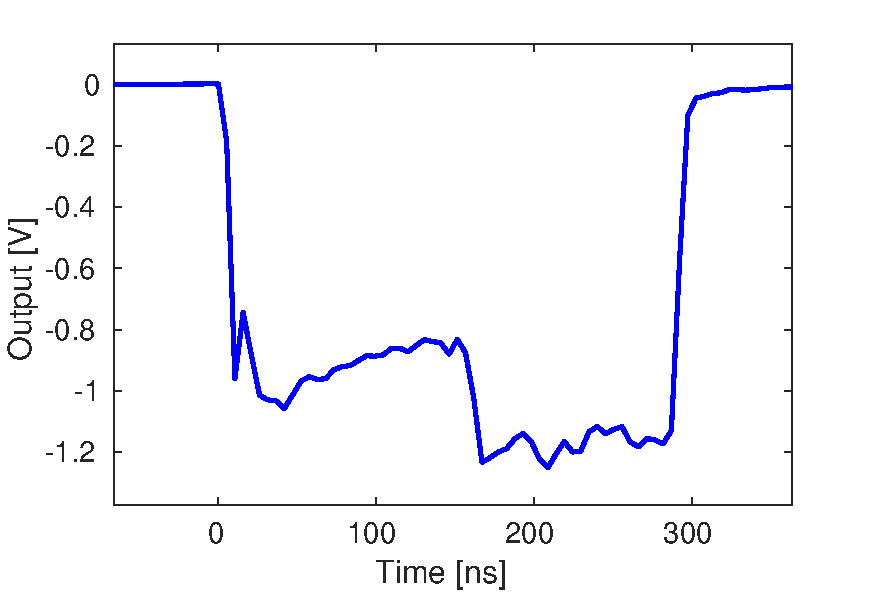
\includegraphics[width=\columnwidth]{figs/hw/phMonBw}
%	\caption{\label{f:phMonBw}
%	}
%\end{figure}

\begin{figure}
	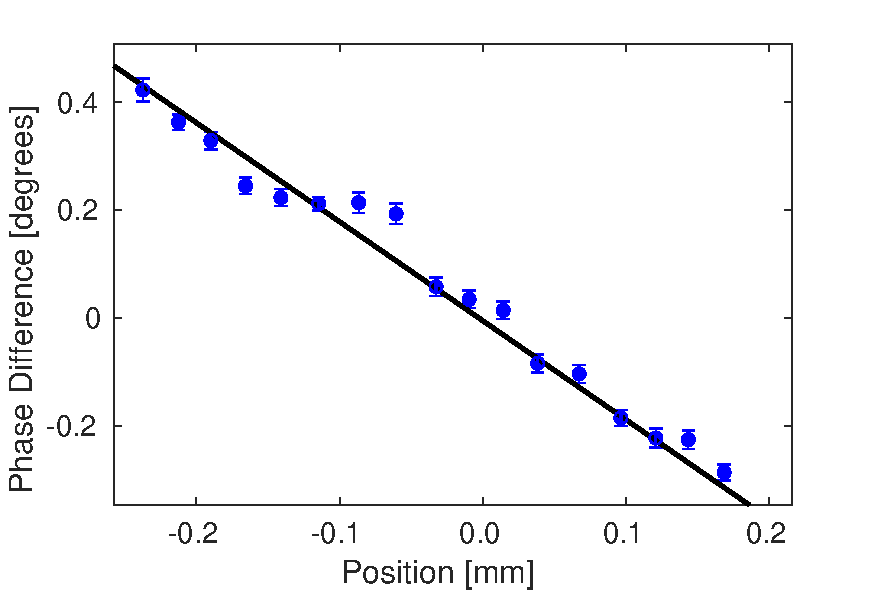
\includegraphics[width=\columnwidth]{figs/hw/phMonHScan}% Here is 
	%how to 
	%import EPS art
	\caption{\label{f:phMonHScan}
	}
\end{figure}

\subsection{\label{ss:font}Feedforward Controller}

% FROM THESIS
The basic logic of the firmware is as follows. The ADC sampling and timing are 
defined by the input trigger and external 357~MHz clock. The ADC outputs are 
processed continuously on the FPGA, including the addition of channel offsets 
and the application of filters. Then the processed ADC~2 (Mixer) output is 
split in two, creating the two parallel strands that become the DAC~1 and DAC~2 
outputs. Note that, instead of using arcsine, the Mixer value is used directly 
in the calculation, thereby assuming the small angle approximation. 
Prior to being sent to the DACs the two output strands are 
multiplied by their corresponding gain factors, as set in the DAQ. An 
additional delay can be added to the DAC outputs, allowing the synchronisation 
of the correction with the beam to be adjusted. The two calculated DAC outputs 
are connected to the amplifier drive inputs, where they are amplified and 
eventually output to the kickers to deflect the beam and correct the phase. 
The overall latency of the FONT5a board, from the arrival of the signal at the 
ADCs to the output of the calculated correction at the DACs, is around 22 clock 
cycles (at 357~MHz) or 60~ns \cite{glennCLIC14}.
% /FROM THESIS

%\begin{figure}
%	\includegraphics[width=\columnwidth]{figs/hw/FONT5aPanel}% Here is 
%	%how to 
%	%import EPS art
%	\caption{\label{f:FONT5aPanel}
%	}
%\end{figure}

\begin{figure}
	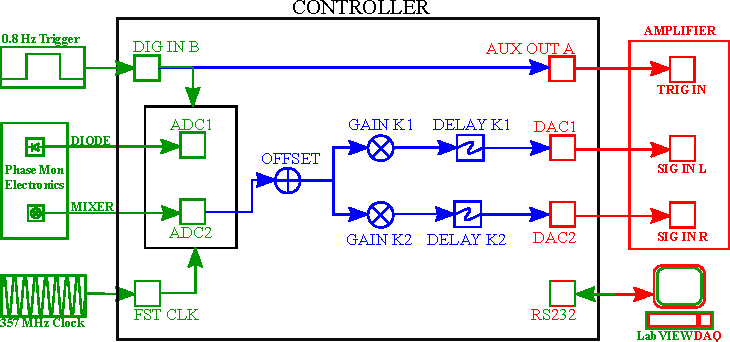
\includegraphics[width=\columnwidth]{figs/hw/fontDiagram}% Here is 
	%how to 
	%import EPS art
	\caption{\label{f:fontDiagram}
	}
\end{figure}

% FROM THESIS
In the PFF system the voltage sent to the kickers in the TL2 chicane (see 
Figures~\ref{f:ctfpffLayout}~and~\ref{f:newTL2Lattice}) is varied depending on 
the upstream phase. The corrected downstream phase, \(\phi_{PFF}\), can 
therefore be simply modelled as subtracting the upstream phase, \(\phi_u\), 
from the initial downstream phase \(\phi_d\):
\begin{equation}
\phi_{PFF} = \phi_d - g\phi_u
\label{e:pffEq1}
\end{equation}
\begin{equation}
g = \rho_{ud}\left(\frac{\sigma_d}{\sigma_u}\right)
\label{e:theoretOptGain}
\end{equation}
\begin{equation}
\sigma_{PFF} = \sigma_d\sqrt{1-\rho_{ud}^2}
\end{equation}
%/FROM THESIS


\subsection{\label{ss:amp}Amplifiers}

% FROM THESIS
The amplifier takes the two DAC signals from the FONT5a board and
uses them to produce four high voltage outputs. These are connected to the 
downstream ends of the kicker strips (two kickers and two strips per kicker 
gives four connections at the downstream ends in total), creating the potential 
difference between the strips that deflects the beam in order to correct the 
phase. The returning signals from the upstream ends of the kicker strips are 
then terminated back at the amplifier.

\begin{figure}
	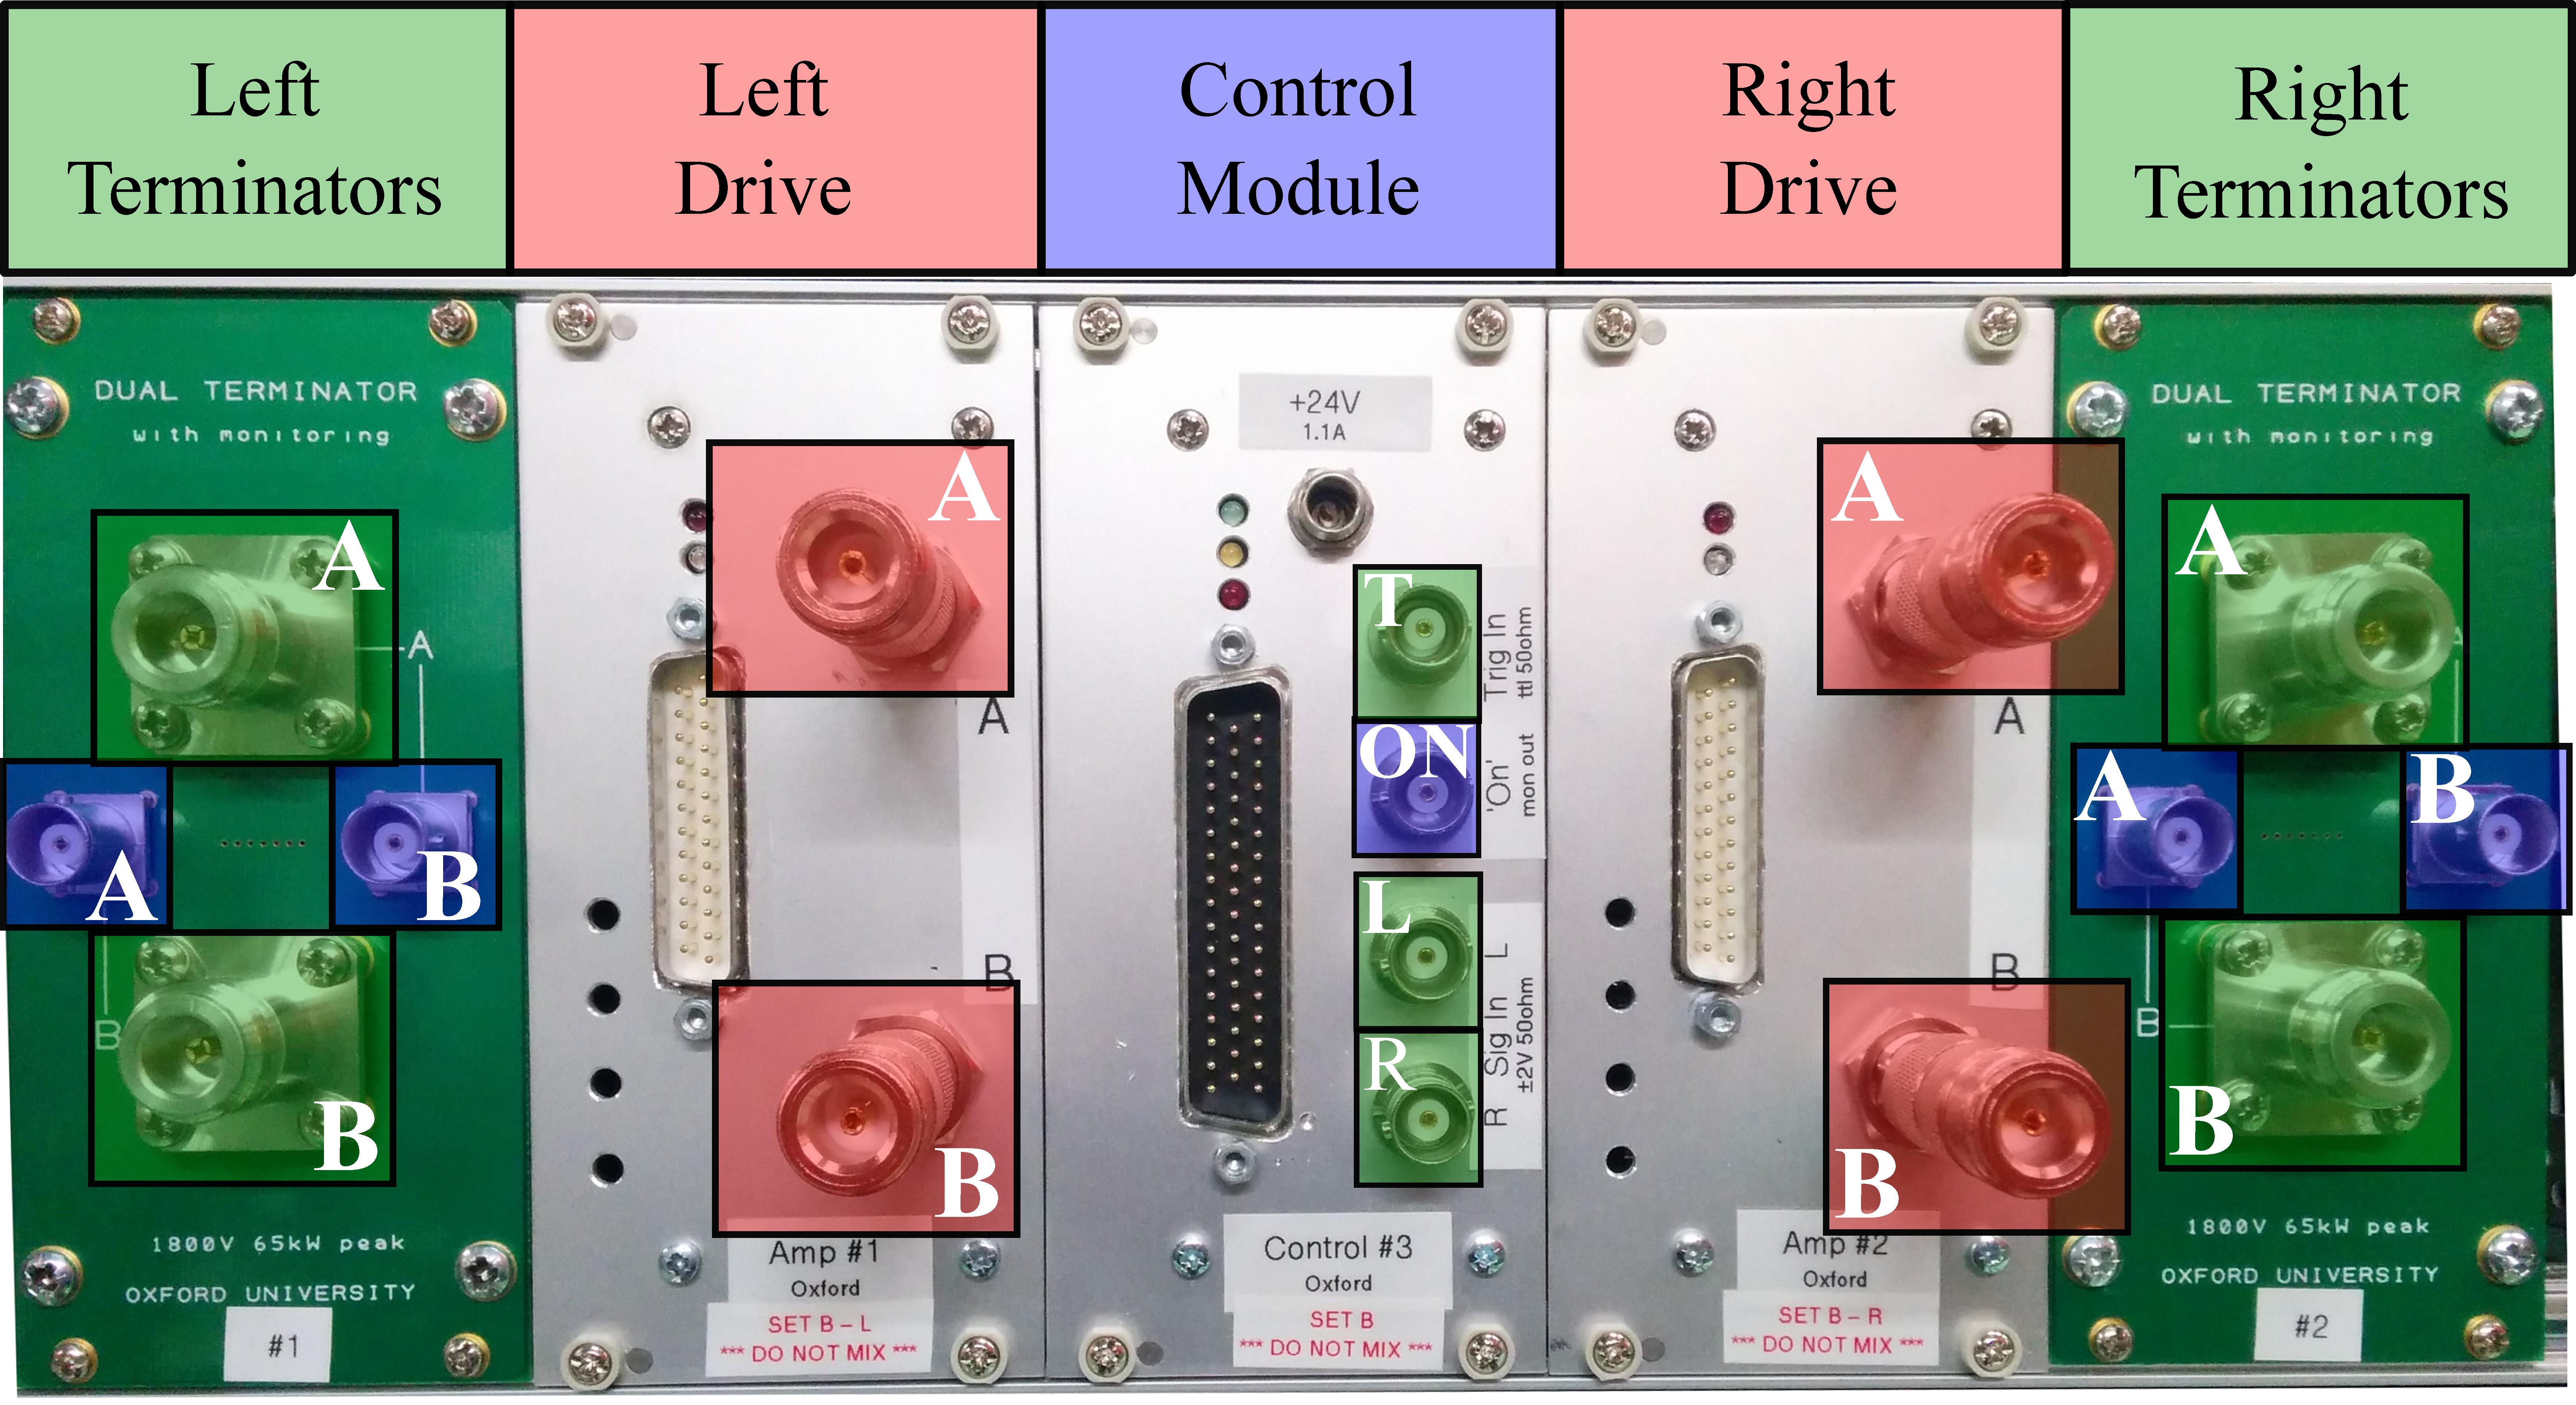
\includegraphics[width=\columnwidth]{figs/hw/AmpPanel}% Here is 
	%how to 
	%import EPS art
	\caption{\label{f:AmpPanel}
	}
\end{figure}

The amplifier is purpose built for the PFF prototype, also at Oxford 
University, with further details of its design available in \cite{colinCLIC16}. 
An annotated picture of its front panel is shown in 
Figure~\ref{f:AmplifierPanelPic} and a simplified diagram showing the flow of 
signals between the FONT5a board, amplifier and kickers is shown in 
Figure~\ref{f:amplifierDiagram}.
The amplifier is installed in a standard 3U rack and has a modular design. It 
consists of five individual modules split between two sides, labelled left and 
right. The left side of the amplifier, which uses the DAC~1 output, powers the 
first kicker in the chicane, and the right side of the amplifier, which uses 
the DAC~2 output, powers the second kicker. Each side of the amplifier contains 
its own ``drive module'' and ``terminator module''. Finally there is a central 
``control module'' that is common to both sides of the amplifier.

\begin{figure}
	\begin{subfigure}{\columnwidth}
		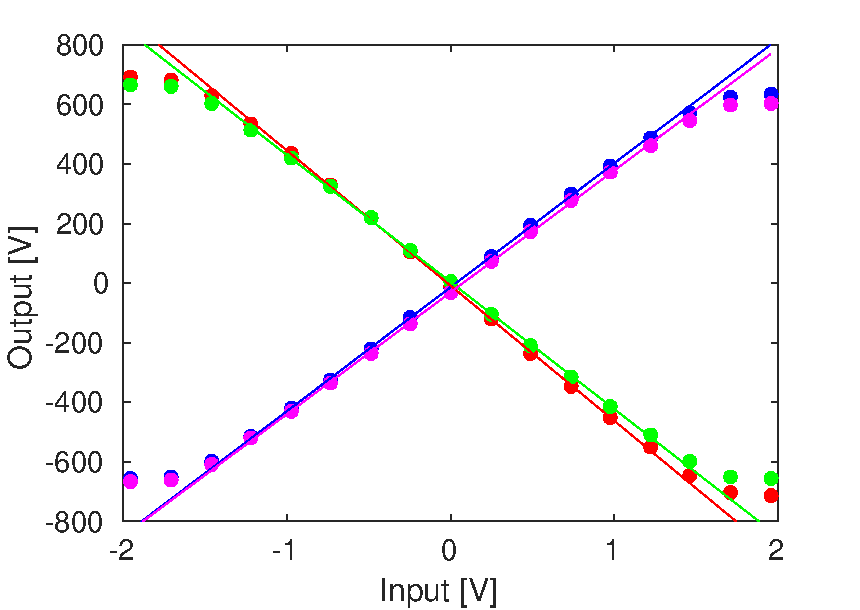
\includegraphics[width=\textwidth]{figs/hw/AmpOutvsDAC}
		\caption{}
		\label{f:AmpOutvsDAC}
	\end{subfigure}

	\begin{subfigure}{\columnwidth}
		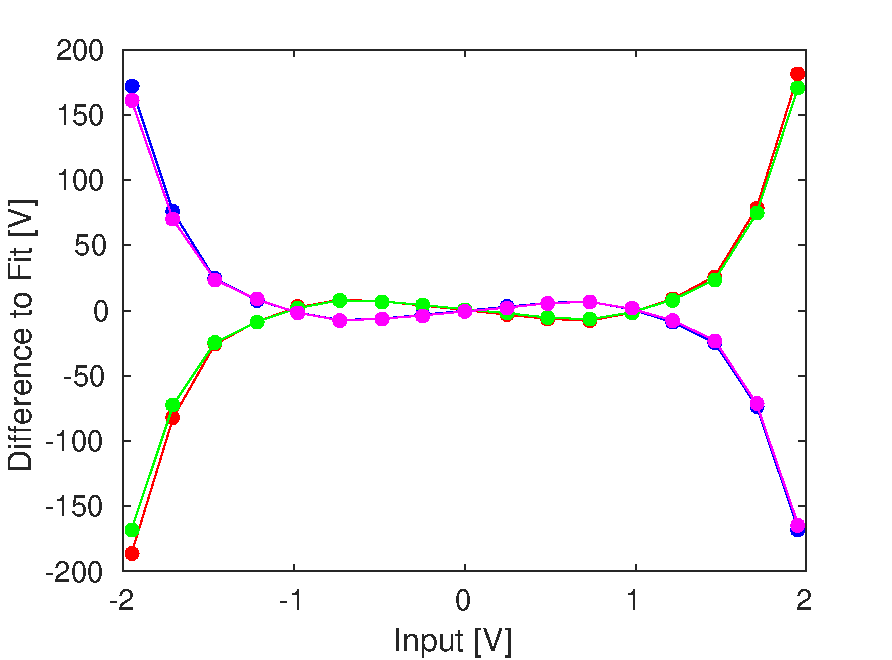
\includegraphics[width=\textwidth]{figs/hw/AmpOutvsDAC_residual}
		\caption{}
		\label{f:AmpOutvsDAC_residual}
	\end{subfigure}	
	\caption{\label{f:AmpOutvsDACFig}test \ref{f:AmpOutvsDAC}}
\end{figure}

Figure~\ref{f:AmpOutvsDAC} shows the amplifier output, measured using the 
monitoring signals, at different constant input voltages sent from the FONT5a 
board between the minimum of -2V (-4095 DAC counts) and maximum of 2V (+4095 
DAC counts). The amplitude of the monitoring signals is converted in to the 
amplifier output voltage using the approximate conversion factor of 115 
\cite{colinPriv}. All four amplifier outputs are shown (one for each strip of 
the two kickers). The values plotted are the mean of the 480~ns central region 
of the whole 1400~ns output pulse.

The response of the amplifier is linear up to \(\pm1.2\)~V input voltage. 
Outside this range the amplifier clearly begins to enter saturation, in 
particular above input voltages of \(\pm1.7\)~V. The linear fits shown include 
only the points up to \(\pm1.2\)~V, in order to not be biased by the effects of 
saturation. Figure \ref{f:AmpOutvsDAC_residual} shows the difference between 
the linear fit and the measured amplifier output across the full range of input 
voltages. A slight deviation from linearity in the \(\pm1.2\)~V range is also 
visible, although the maximum difference is only 10~V or a 3\% relative error.

Figures~\ref{f:ampLTraces} and \ref{f:ampRTraces} show the full 
1.4~\(\mathrm{\mu}\)s amplifier output with a constant input of \(+1\)~V 
(\(-1\)~V) applied to the left (right) amplifier respectively. Spikes in the 
signal just prior to 2000~ns and after 3000~ns on the time axis as seen in the 
plots are pickup on the kicker strips induced by the beam. For a constant input 
voltage the output voltage along the pulse varies by up to 88~V peak-to-peak 
(mean 12~V) for the left amplifier or 93~V peak-to-peak (mean 14~V) for the 
right amplifier. As a relative difference, this corresponds to approximately a 
6~\% peak-to-peak, or 1~\% mean, variation along the pulse.
% / FROM THESIS

Brief design

Linearity

Pulse shape

\begin{figure}
	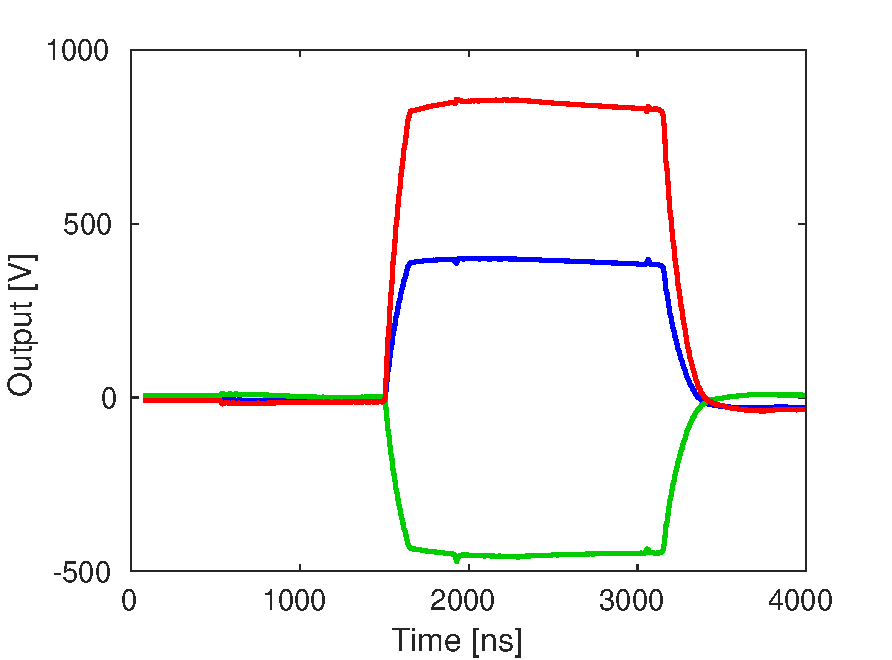
\includegraphics[width=\columnwidth]{figs/hw/AmpL_Traces}% Here is 
	%how to 
	%import EPS art
	\caption{\label{f:AmpL_Traces}
	}
\end{figure}

\subsection{\label{ss:kick}Kickers}

% FROM THESIS
The two electromagnetic kickers provide the phase correction in the PFF system 
by deflecting the beam on to longer or shorter paths in the TL2 chicane (see 
Figure~\ref{f:ctfpffLayout}). They have been designed and built by INFN, Italy 
\cite{infn}, based on a similar design used at the DA\(\mathrm{\Phi}\)NE 
collider \cite{dafneKick}. A schematic of the kicker design is shown in 
Figure~\ref{f:kickerSchematic}. It consists of two parallel conducting strips 
placed along the left and right side of the beam pipe. Each strip is 
approximately one metre in length and the horizontal separation between the 
strips is 40~mm. The strips are tapered at their ends to reduce coupling 
impedance (to reduce the voltage induced on the strips by the beam) 
\cite{kickerIPAC11}.
% /FROM THESIS

Brief design, cable connections etc.

\begin{figure}
	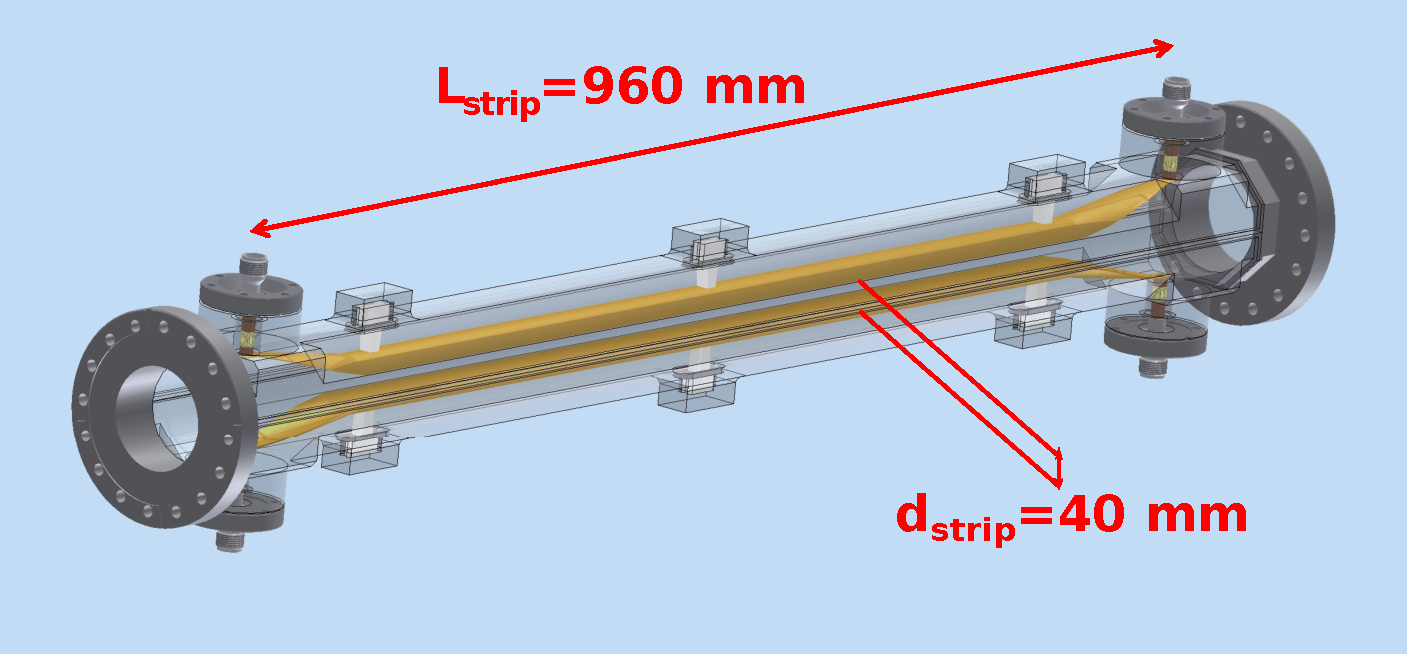
\includegraphics[width=\columnwidth]{figs/hw/kickerSchematic}% Here is 
	%how to 
	%import EPS art
	\caption{\label{f:kickerSchematic}
	}
\end{figure}

\section{\label{s:optics}Optics}

\subsection{\label{ss:chicane}Correction Chicane}

The PFF system places new constraints on the optics of the correction chicane, 
the lattice of which is shown in Fig.~\ref{f:TL2Lattice}. The chicane has a 
dog-leg shape containing 
4 dipoles, with the external pair (B1 and B4) bending the beam through 
\(\pm31^\circ\) and 
the internal pair (B2 and B3) through \(\pm17^\circ\). Each section of the 
chicane between 
the dipoles includes a triplet of quadrupoles. The total length of the chicane, 
including the quadrupole triplet upstream of B1, is around 15~m.

\begin{figure}
	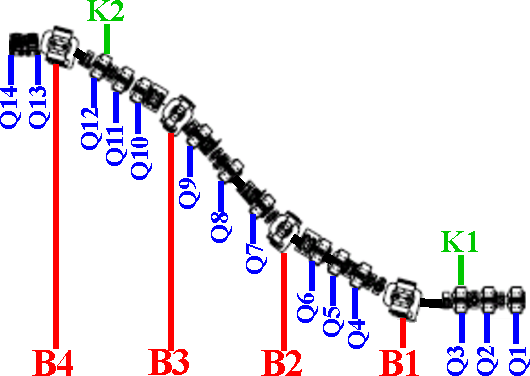
\includegraphics[width=\columnwidth]{figs/optics/TL2Lattice_chicaneOnly}% 
	%Here is 
	%how to 
	%import EPS art
	\caption{\label{f:TL2Lattice}
	}
\end{figure}

The pre-existing TL2 chicane was already densely packed with magnets, and to 
maintain the functionality of the lattice for routine operation at CTF3 
elements could not be removed.
Space for the two PFF kickers (K1 and K2) was made available by rearranging 
quadrupoles in the line, moving quadrupoles with a wide aperture (Q3 and Q12) 
prior to the first (B1) and last (B4) dipole in the chicane.
The kickers are installed inside the aperture of these quadrupoles 
(Fig.~\ref{f:kickerInsideQuad}). 

\begin{figure}
	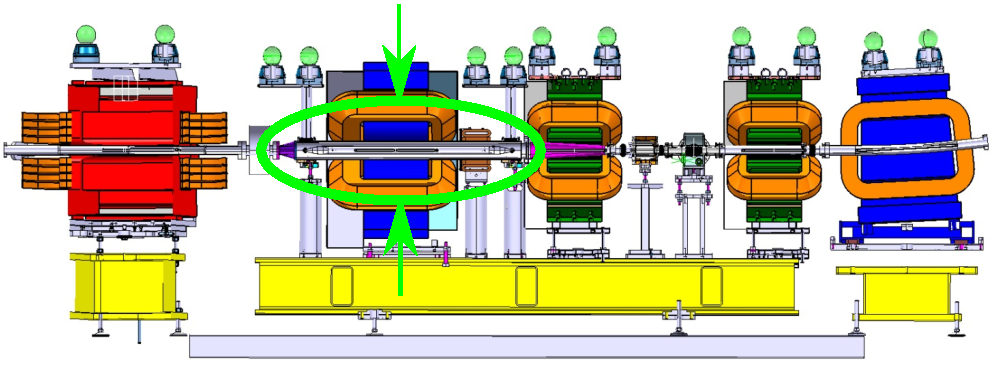
\includegraphics[width=\columnwidth]{figs/optics/kickerInsideQuad}% Here is 
	%how to 
	%import EPS art
	\caption{\label{f:kickerInsideQuad}
	}
\end{figure}

New optics for the TL2 line, maintaining the previous matching constraints 
required for normal operation and adding the new PFF constraints, were created 
using the CTF3 MADX model. The accuracy of the model for the rearranged line 
was verified and improved in a series of kick-response measurements [REF]. 
Relying on the pre-existing chicane layout forced several compromises in the 
chicane optics.

The original optics constraints include - matching combiner ring extraction and 
CLEX injection, dispersion closure and minimised, beta functions small/smooth. 
The additional PFF constraints ensure the phase (path length) dependence on the 
kicker voltages, and that the beam orbit downstream of the chicane is closed.

The rms beam energy spread at CTF3 is at the 1\% level. The beam pipe in the 
correction chicane has a diameter of 10~cm to give a large acceptance for the 
dispersion component of the beam size. However, the aperture of the PFF kickers 
is only 2~cm. The dispersion must be closed at the chicane exit and minimised 
at \(K_2\) (\(K_1\) is prior to the chicane in a dispersion free region). 

The correction range of the PFF system, or the dependence of the beam phase on 
the angular deflection applied at \(K_1\), is defined by the transfer matrix 
coefficient \(R_{52}\) between the two kickers:
\begin{equation}
\phi_{\mathrm{K2}} = \phi_i + R_{52}x'_{\mathrm{K1}}
\end{equation}
Maximising \(R_{52}\) has the 
unfortunate consequence of increasing the dispersion, thus the optics must be a 
compromise that achieves a reasonable
correction range whilst keeping the dispersion small enough to avoid beam 
losses.

The dispersion and phase shift for a 1~mrad kick at \(K_1\) in the matched 
optics for the chicane are shown in Fig.[REF] and Fig.[REF] respectively. An 
\(R_52\) value of 0.74~m 
is achieved (corresponding to a phase shift of \(-10.6^\circ\) per mrad at 
\(K_1\)) with 
a dispersion of [val] at \(K_2\). With this dispersion approximately [val] 
sigma of the beam energy distribution fits within the \(K_2\) aperture.

\begin{figure*}
	\begin{subfigure}{\columnwidth}
		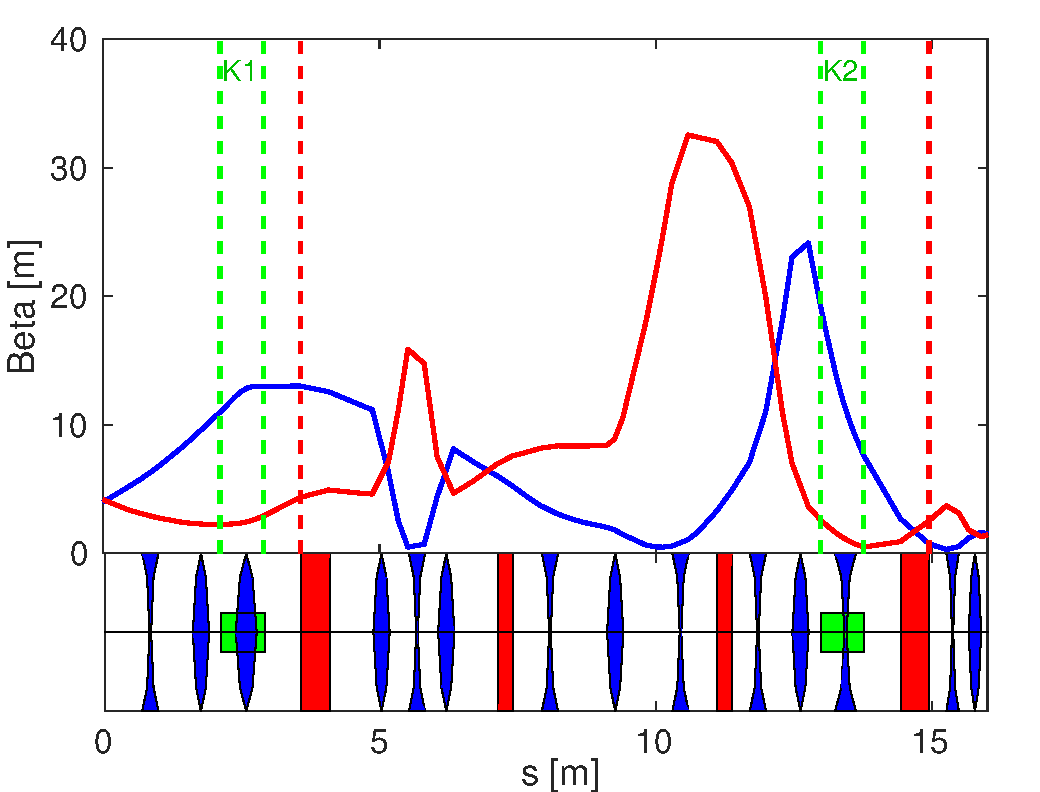
\includegraphics[width=\textwidth]{figs/optics/pffOpticsBeta_chicane}
		\caption{}
		\label{f:pffOpticsBeta}
	\end{subfigure}
	\begin{subfigure}{\columnwidth}
		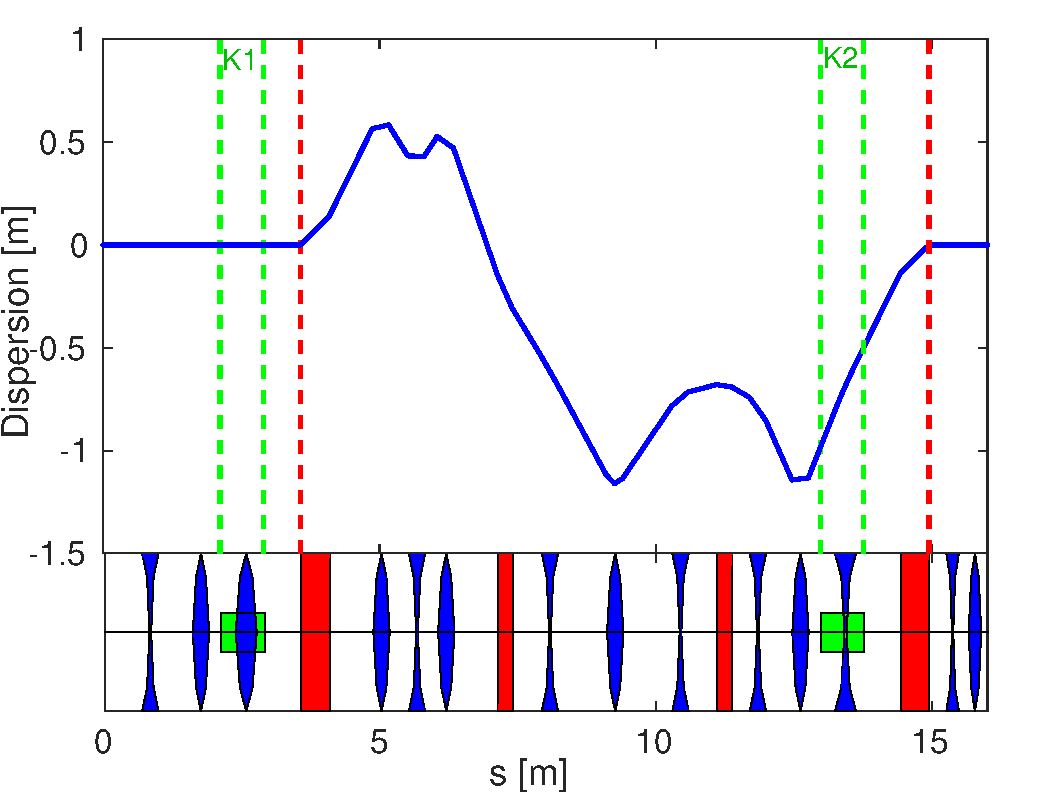
\includegraphics[width=\textwidth]{figs/optics/pffOpticsDisp_chicane}
		\caption{}
		\label{f:pffOpticsDisp_chicane}
	\end{subfigure}

	\begin{subfigure}{\columnwidth}
		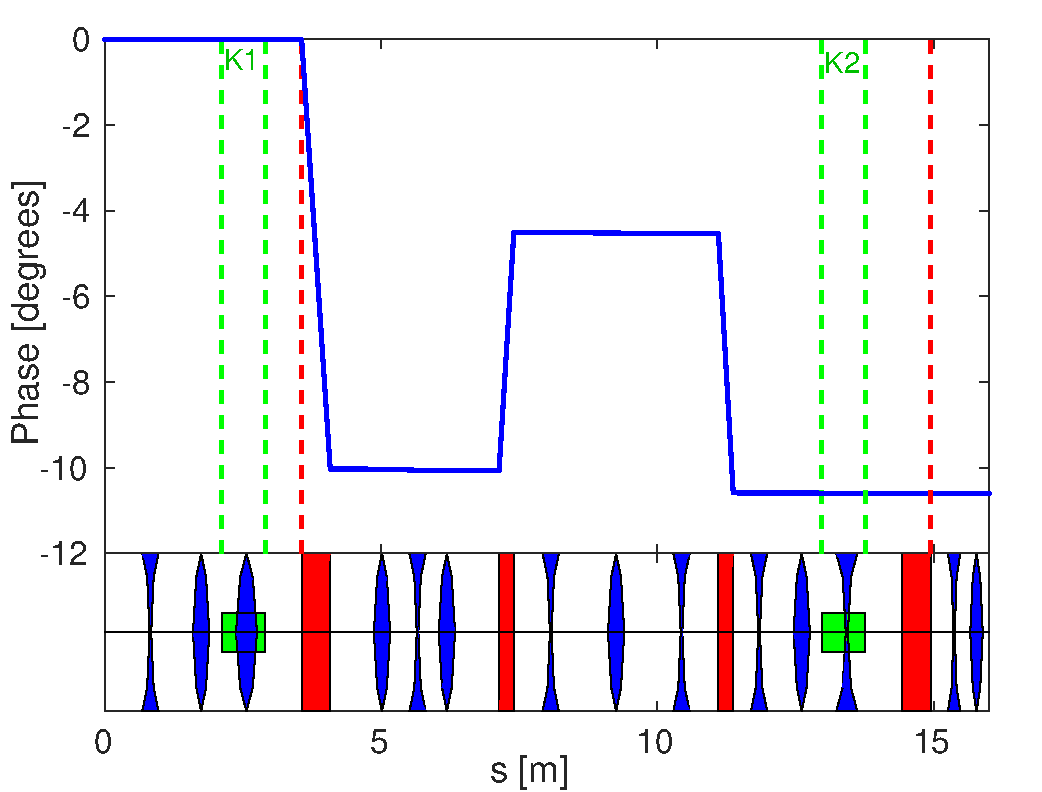
\includegraphics[width=\textwidth]{figs/optics/pffOpticsPhase_chicane}
		\caption{}
		\label{f:pffOpticsPhase_chicane}
	\end{subfigure}
	\begin{subfigure}{\columnwidth}
		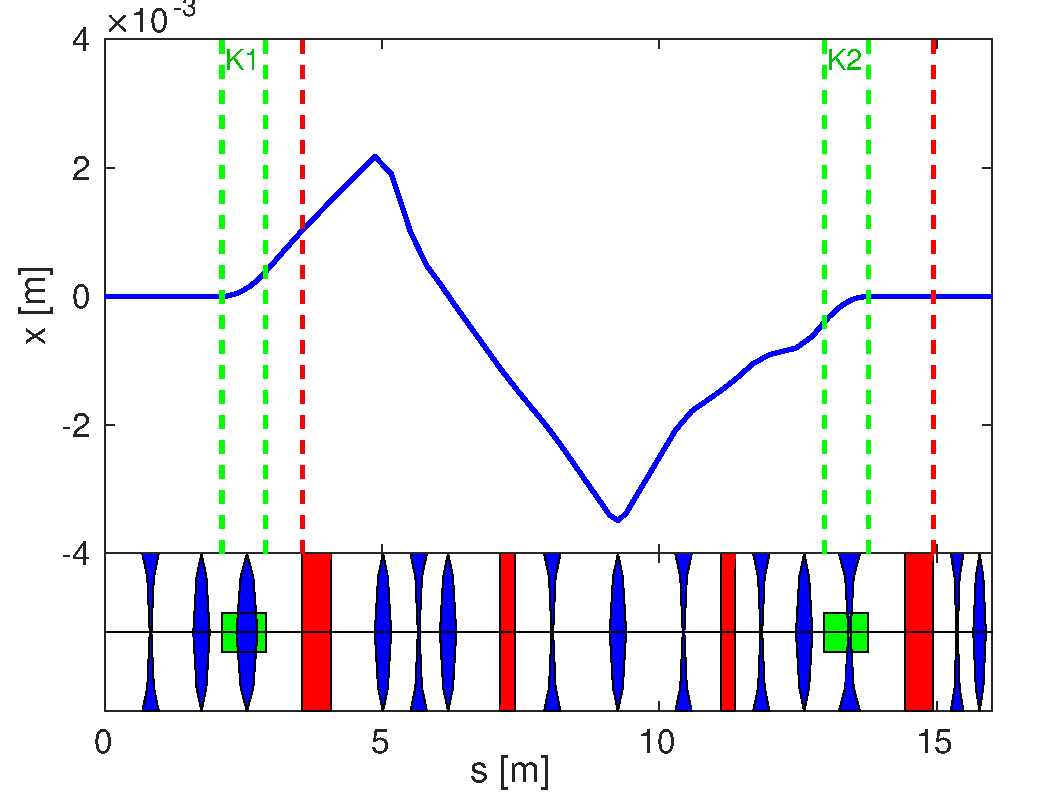
\includegraphics[width=\textwidth]{figs/optics/pffOpticsX_chicane}
		\caption{}
		\label{f:pffOpticsX_chicane}
	\end{subfigure}

	\begin{subfigure}{\columnwidth}
		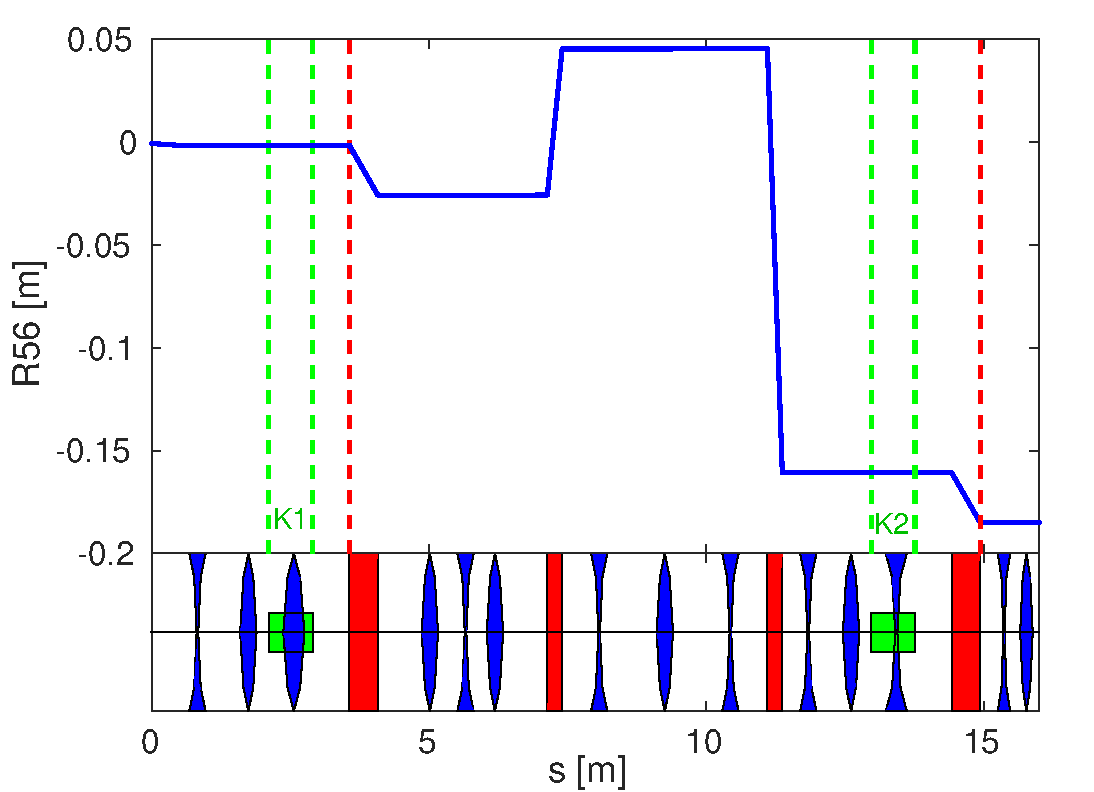
\includegraphics[width=\textwidth]{figs/optics/pffOpticsR56_chicane}
		\caption{}
		\label{f:pffOpticsR56_chicane}
	\end{subfigure}

	\caption{\label{f:opticsPlots}Optics for the correction chicane.}

\end{figure*}

The last two figures, \ref{f:pffOpticsX}~and~\ref{f:pffOpticsPhase}, show the 
effect of kicking the beam with the PFF kickers. A deflection of +1~mrad is 
applied from the first kicker, and -1~mrad from the second kicker. This leads 
to a peak horizontal orbit offset of 3.5~mm inside the horizontal chicane. The 
orbit is closed at the \(10^{-7}\) level following the chicane, so that the 
beam's trajectory following the PFF system is independent of the applied kick. 

Finally, the \(R_{52}\) value between the two kickers is 0.74~m. This defines 
the phase shift resulting from kicking the beam in the chicane, which is the 
key figure of merit for the PFF system. As shown in 
Figure~\ref{f:pffOpticsPhase} a kick of 1~mrad provides a phase shift of 
\(-10.6^\circ\) in this optics. This is converted in to the actual range of the 
PFF system taking in to account the specifications of the kicker amplifiers in 
Chapter~\ref{c:commissioning}. Verifications of the performance of the optics 
are presented in Chapters~\ref{c:phasePropagation}~and~\ref{c:commissioning}.
% /FROM THESIS

\subsection{\label{ss:prop}Phase Propagation}

As in Eq.[ref] the corrected downstream phase jitter that the PFF system can 
achieve depends on the correlation between the upstream (input) phase and the 
initial downstream phase. This correlation is determined by the phase monitor 
resolution and any additional beam phase jitter introduced in-between 
\(\phi_u\) and \(\phi_d\). In the first measurements with the new correction 
chicane optics (such as Fig.\ref{f:origUpVsDown}) the correlation was below 
40\% and the downstream phase jitter more than two times larger than upstream. 

\begin{figure}
	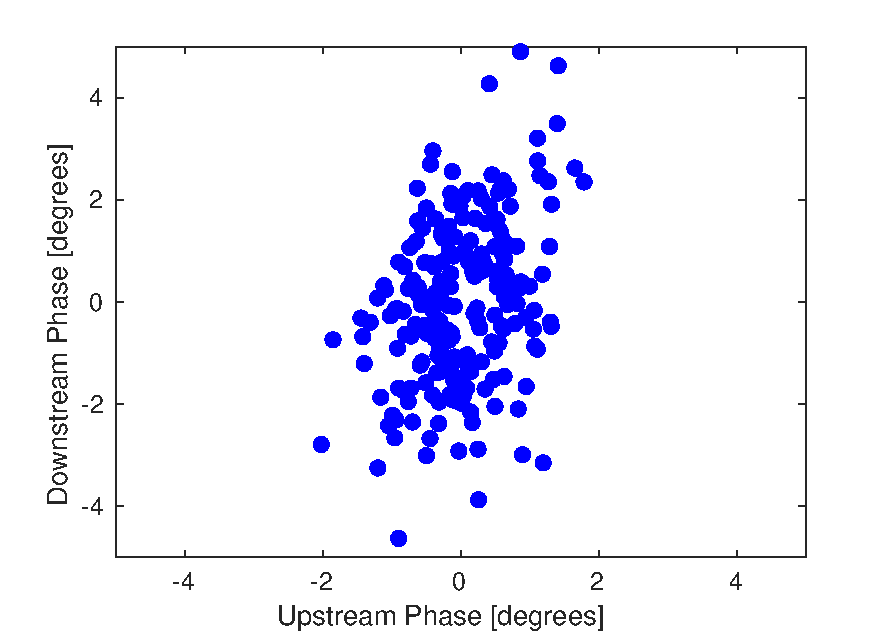
\includegraphics[width=\columnwidth]{figs/prop/origUpVsDown}% Here is 
	%how to 
	%import EPS art
	\caption{\label{f:origUpVsDown}
	}
\end{figure}

% FROM THESIS
One constraint that could not be met in conjunction with the other chicane 
optics requirements was for the transfer matrix element \(R_{56}\) to be zero. 
\(R_{56}\) describes the dependence of the phase on the beam energy, to first 
order, as 
follows: 
\begin{equation}
\phi_d = \phi_u + R_{56}\frac{\Delta p}{p}
\label{e:r56PhasEq}
\end{equation}
Where \(R_{56}\) is the \(R_{56}\) coefficient between the upstream and 
downstream monitors, and \(\Delta p/p\) is the fractional energy offset.

As seen in Figure~\ref{f:pffOpticsR56} the \(R_{56}\) transfer matrix 
coefficient across the horizontal chicane is -0.18~m. As other beam lines at 
CTF3 nominally have \(R_{56}=0\), the total \(R_{56}\) between \(\phi_u\) and 
\(\phi_d\) is also -0.18~m. This leads to additional energy dependent phase 
jitter in \(\phi_d\) that is not present in \(\phi_u\).

\begin{figure}
	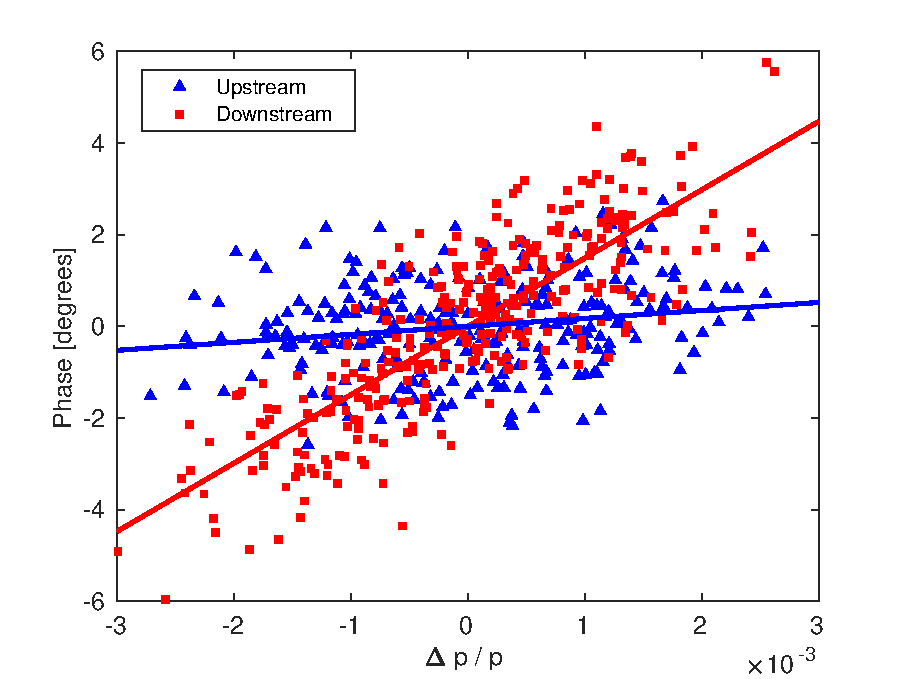
\includegraphics[width=\columnwidth]{figs/prop/UpDownEnCorr}
	\caption{\label{f:UpDownEnCorr}
	}
\end{figure}

The effect of this is shown in Fig.~\ref{f:UpDownEnCorr}, in which the phase is 
plotted versus the beam energy (calculated using the beam position in a 
dispersive BPM). A correlation of [val] between the upstream phase and the beam 
energy is amplified to [val] downstream.

From Equations [val] and [val] the effect of \(R_{56}\) on the correlation and 
the PFF performance can be derived [REF]. Excluding the phase monitor 
resolution, the 
corrected downstream phase jitter that can be achieved is given by:
% FROM THESIS
%\begin{equation}
%\rho_{ud} = \frac{\sigma_u + R_{56}\rho_{up}\sigma_p}{\sqrt{\sigma_u^2 + 
%		R_{56}^2\sigma_{p}^2 + 2R_{56}\rho_{up}\sigma_{u}\sigma_{p}}}
%\label{e:r56CorrDefFinal}
%\end{equation}
\begin{equation}
\sigma_{PFF} = \left|R_{56}\right|\sigma_p\sqrt{1-\rho_{up}^2}
\label{e:r56PFFJit}
\end{equation}
Where \(\sigma_p\) is the beam energy jitter (typically [val] at CTF3) and 
\(\rho_{up}\) is the correlation between the upstream phase and the beam energy 
(typically [val]). Fig.\ref{f:jitVsR56} shows the dependence of the initial and 
corrected downstream phase jitter on the \(R_{56}\) value. The slight asymmetry 
between positive and negative \(R_{56}\) values is caused by the non-zero 
correlation between the upstream phase and the beam energy. To reduce a typical 
initial beam jitter of \(0.8^\circ\) at CTF3 to the CLIC target of 
\(0.2^\circ\), the \(R_{56}\) value between the upstream and downstream 
monitors must be less than [val].

%\begin{figure}
%	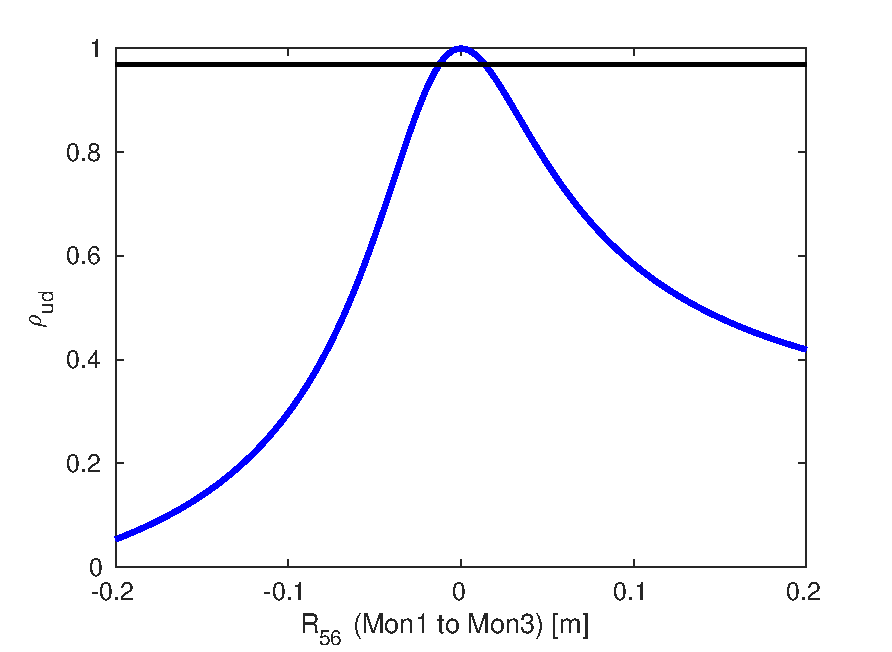
\includegraphics[width=\columnwidth]{figs/prop/corrVsR56}
%	\caption{\label{f:corrVsR56}
%	}
%\end{figure}
\begin{figure}
	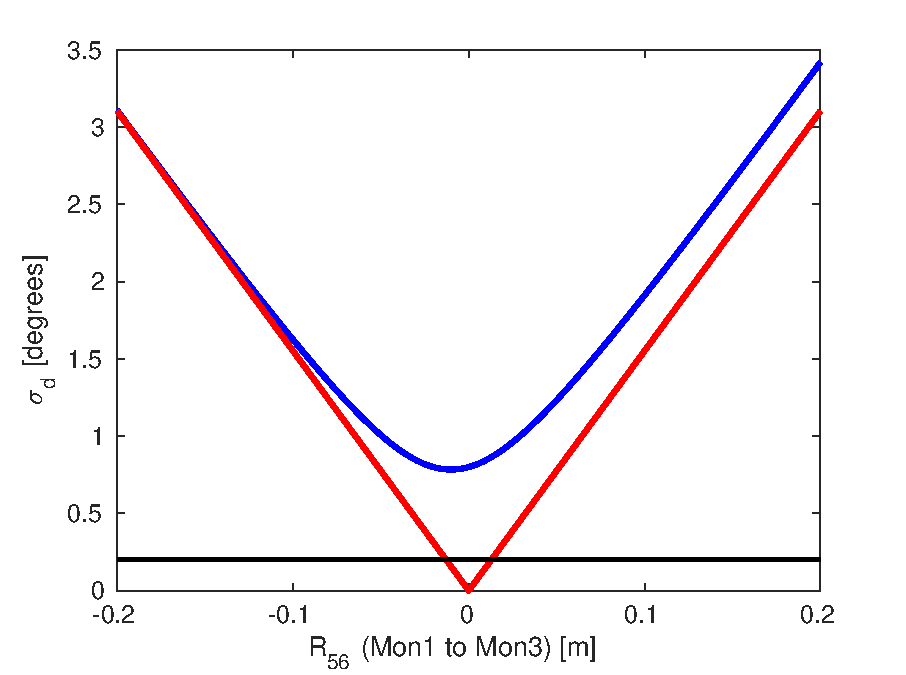
\includegraphics[width=\columnwidth]{figs/prop/jitVsR56}
	\caption{\label{f:jitVsR56}
	}
\end{figure}


To compensate, messed around with TL1... R56 scan...

Optimal \(R_{56}\) value not constant... correlation variations along pulse... 
hinted at higher order effects... Second order phase-energy dependence in the 
optics is described using the \(T_{566}\) matrix coefficient:
\begin{equation}
\phi_d = \phi_u + R_{56}\left(\frac{\Delta p}{p}\right) + 
T_{566}\left(\frac{\Delta p}{p}\right)^2
\label{e:t566}
\end{equation}

%\begin{equation}
%R_{56} = -2T_{566} \left(\frac{\Delta p}{p}\right)
%\label{e:r56t566dep}
%%\end{equation}
%/FROM THESIS

% FROM THESIS
Fig.~\ref{f:R56ScanGunWiggle_PhaseVsEnergy} shows the dependence of the mean 
downstream phase on the beam energy for three different \(R_{56}\) values set 
in TL1: \(-0.1\)~m, \(0.075\)~m and \(0.3\)~m. The beam energy was varied 
during the data taking period, and the second order term becomes clear.
% /FROM THESIS


%\begin{figure}
%	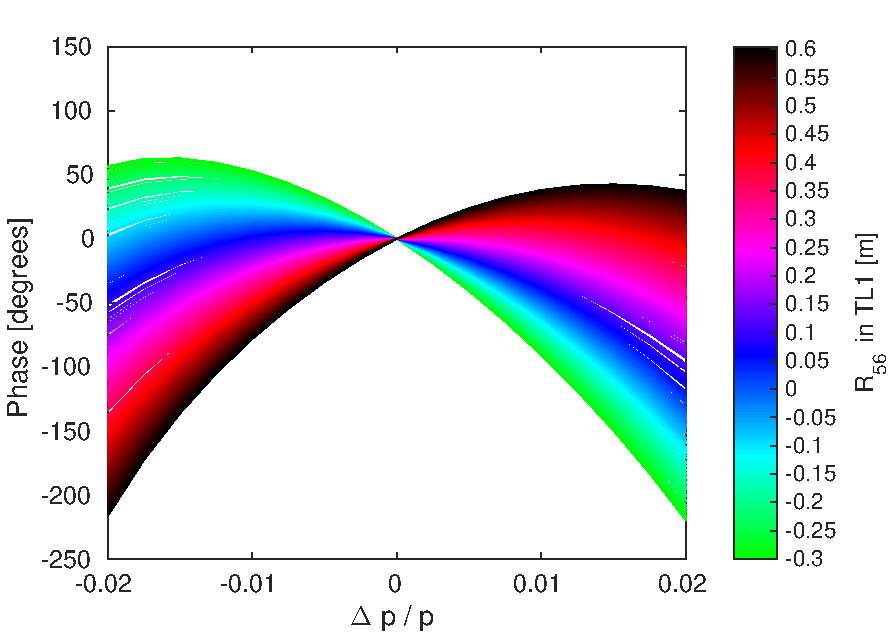
\includegraphics[width=\columnwidth]{figs/prop/phaseVsEn_t566}% Here is 
%	%how to 
%	%import EPS art
%	\caption{\label{f:phaseVsEn_t566}
%	}
%\end{figure}

\begin{figure}
	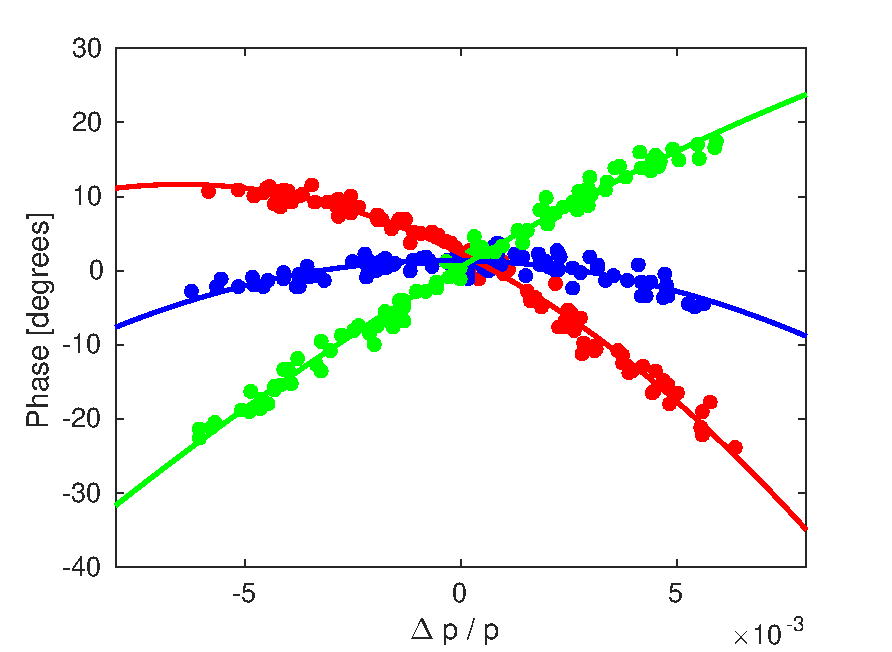
\includegraphics[width=\columnwidth]{figs/prop/R56ScanGunWiggle_PhaseVsEnergy}%
	% Here is 
	%how to 
	%import EPS art
	\caption{\label{f:R56ScanGunWiggle_PhaseVsEnergy}
	}
\end{figure}

Figs.~\ref{f:corrVsEnergyOffset}~and~\ref{f:maxCorrWithT566} shows the effect 
of \(T_{566}\) on the correlation for different beam energy offsets and beam 
energy jitters respectively. In each case it is assumed the first order 
\(R_{56}\) has been completely cancelled using TL1. energy jitter/offset [val] 
assumed.

\begin{figure*}
	\begin{subfigure}{\columnwidth}
		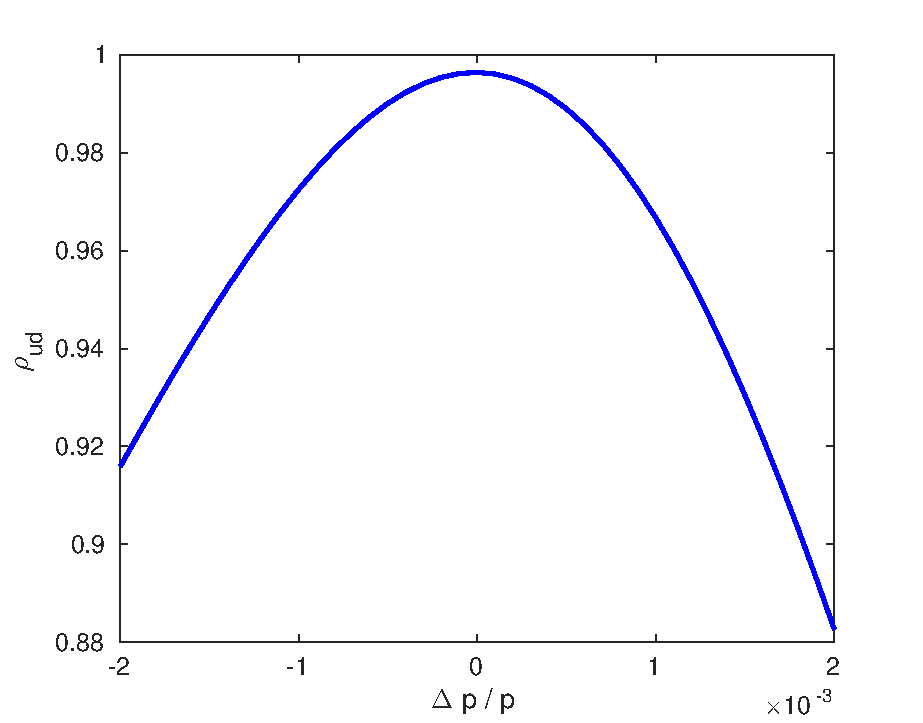
\includegraphics[width=\textwidth]{figs/prop/corrVsEnergyOffset}
		\caption{}
		\label{f:corrVsEnergyOffset}
	\end{subfigure}
	\begin{subfigure}{\columnwidth}
		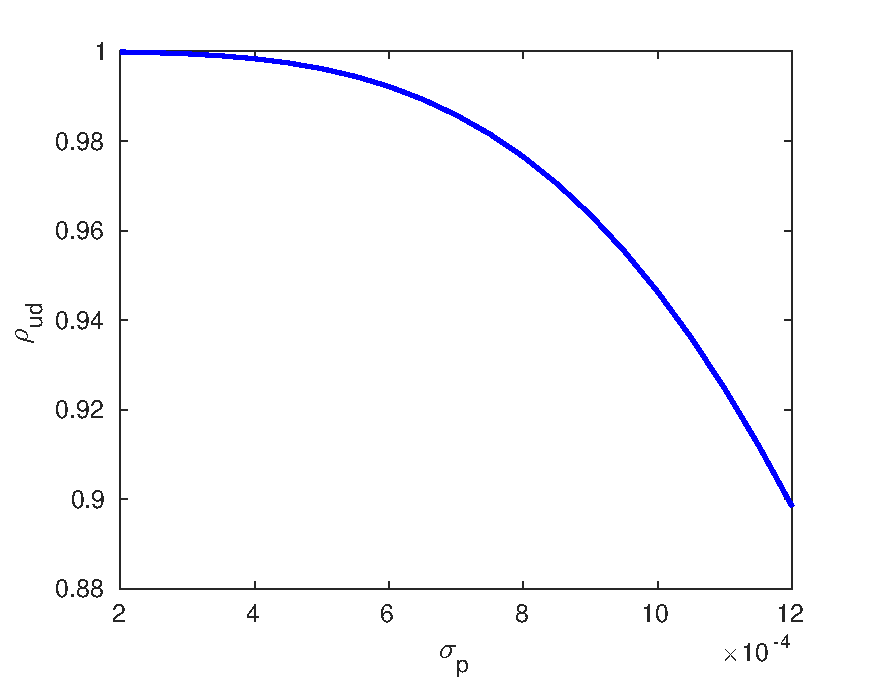
\includegraphics[width=\textwidth]{figs/prop/maxCorrWithT566}
		\caption{}
		\label{f:maxCorrWithT566}
	\end{subfigure}
\end{figure*}

In optimal conditions CTF3 energy jitter as low as [val] and variations along 
pulse below [val], which means not a limiting factor to achieve 0.2 degrees. 
But the sensitivity to energy drifts made it difficult/impossible to maintain 
peak PFF performance on long time scales. CLIC application would require 
\(R_{56}\) and \(T_{566}\) to be zero in the turnarounds.

\section{\label{s:verify}System Setup and Verification}

\subsection{\label{ss:corrRange}Correction Range}

% FROM THESIS
Figure \ref{f:phaseVsAmpVoltage} shows the measured mean phase shift in the 
downstream phase monitor across the full \(\pm2\)~V input range of the 
amplifier. Constant DAC outputs in 17 steps between -4095 counts (-2~V) and 
+4095 counts (+2~V) were used to drive the amplifier. For each amplifier input 
voltage 100 beam pulses were acquired in interleaved mode in order to reduce 
the sensitivity to any drifts in beam phase between data points. The phase 
plotted in Figure~\ref{f:phaseVsAmpVoltage} is the difference between the 50 
beam pulses with the DAC output enabled (non-zero amplifier input) and the 50 
beam pulses with the DAC output disabled (0~V amplifier input).
At the maximum amplifier input voltage of \(2\)~V the phase is shifted by 
\(5.5\pm0.3^\circ\). The fitted phase shift per Volt input is 
\(3.5\pm0.1^\circ\) in the \(\pm1.2\)~V linear range of the amplifier.
% /FROM THESIS

\begin{figure}
	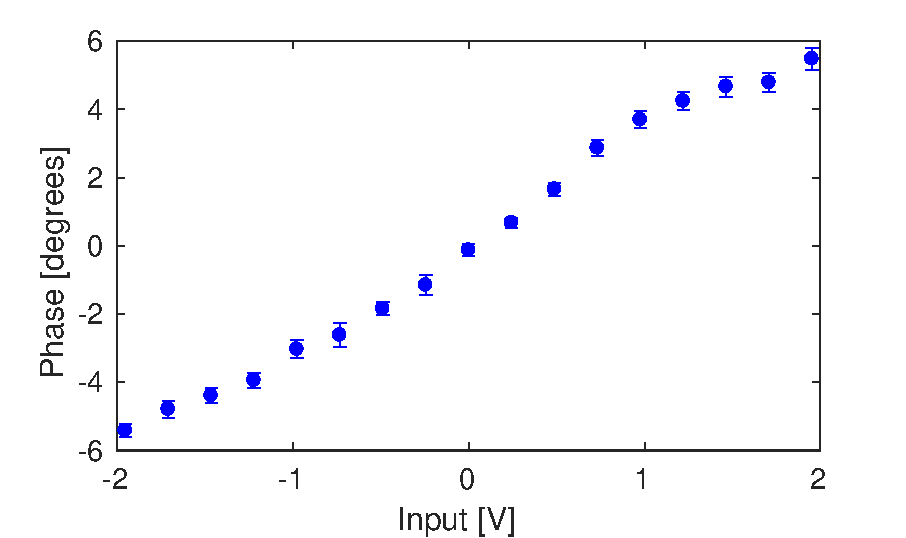
\includegraphics[width=\columnwidth]{figs/optics/corrRange} 
	\caption{\label{f:corrRange}
	}
\end{figure}

The measured correction range is shown in Fig.\ref{f:corrRange}.
Correction range agrees with expected range

Correction shape

% FROM THESIS
In the central region of the pulse all three traces have the same shape as 
expected. The upstream phase and DAC output should be close to identical by 
definition, as the calculated correction output is only dependent on the input 
phase, but this verifies the functionality of the FONT5a board correction 
algorithm and firmware. The agreement in shape of the downstream phase shift is 
a significant achievement, and verifies the linearity of the amplifier output, 
kicker response and optics for a varying input voltage. This result 
demonstrates that everything is in place for the PFF prototype to flatten 
variations in the downstream phase and to reduce the downstream phase jitter.

The agreement in shape holds for times between around 900~ns and 1375~ns as 
indicated on the figure, and this defines a 475~ns portion of the pulse within 
which the applied correction should be close to optimal. Outside this range the 
large phase sag along the pulse leads 
to the correction being saturated -- the maximum possible DAC output 
(2~V) is applied and the shape can no longer be corrected. It can also
be seen that the measured downstream phase shift saturates earlier than
the applied DAC output. This is because the amplifier begins to 
saturate at input voltages below 2~V, as seen in Figure~\ref{f:AmpOutvsDAC}.
% /FROM THESIS

\subsection{\label{ss:corrShape}Correction Shape}

The PFF system removes intra-pulse phase variations as well as inter-pulse 
variations. 

The input upstream phase, calculated DAC output and the observed difference in 
the downstream phase resulting from the applied kick are all shown. The 
downstream phase trace shows the difference between subsequent pulses with the 
correction on and off (using the interleaved correction mode). 
Each trace is scaled, aligned in time and sign flipped where appropriate to 
make a comparison between the shapes easier.

In the central region of the pulse all three traces have the same shape as 
expected. This verifies the linearity of the amplifier output, kicker response 
and optics for a varying input voltage. This result demonstrates that 
everything is in place for the PFF prototype to flatten variations in the 
downstream phase and to reduce the downstream phase jitter.

The agreement in shape holds for times between around 900~ns and 1375~ns as 
indicated on the figure, and this defines a 475~ns portion of the pulse within 
which the applied correction should be close to optimal. Outside this range the 
large phase sag along the pulse leads 
to the correction being saturated -- the maximum possible DAC output 
(2~V) is applied and the shape can no longer be corrected. It can also
be seen that the measured downstream phase shift saturates earlier than
the applied DAC output. This is because the amplifier begins to 
saturate at input voltages below 2~V, as seen in Figure~\ref{f:AmpOutvsDAC}.

\begin{figure}
	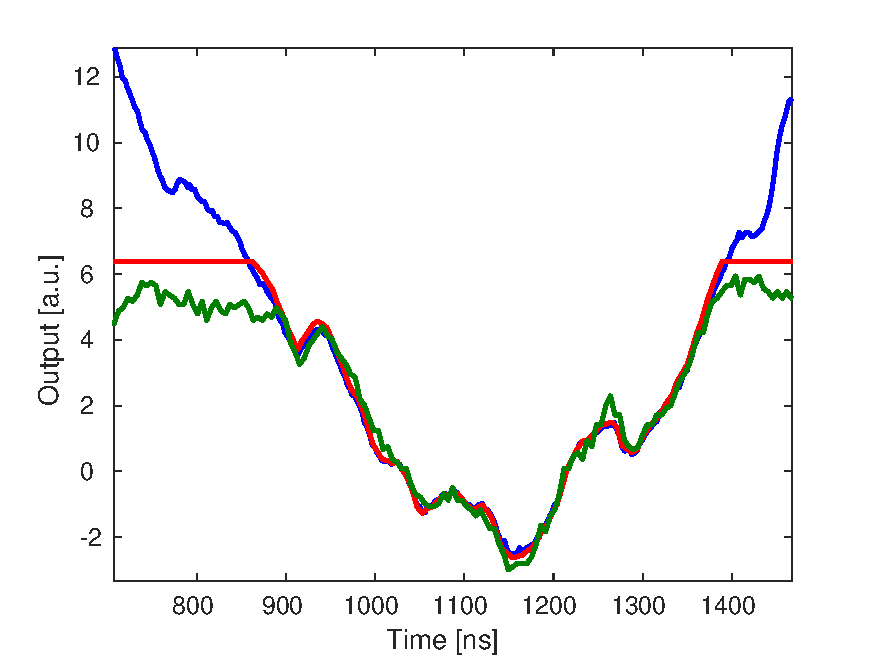
\includegraphics[width=\columnwidth]{figs/comis/pffKickShape} 
	\caption{\label{f:pffKickShape}
	}
\end{figure}

\subsection{\label{ss:orbClos}Orbit Closure}

\begin{figure}
	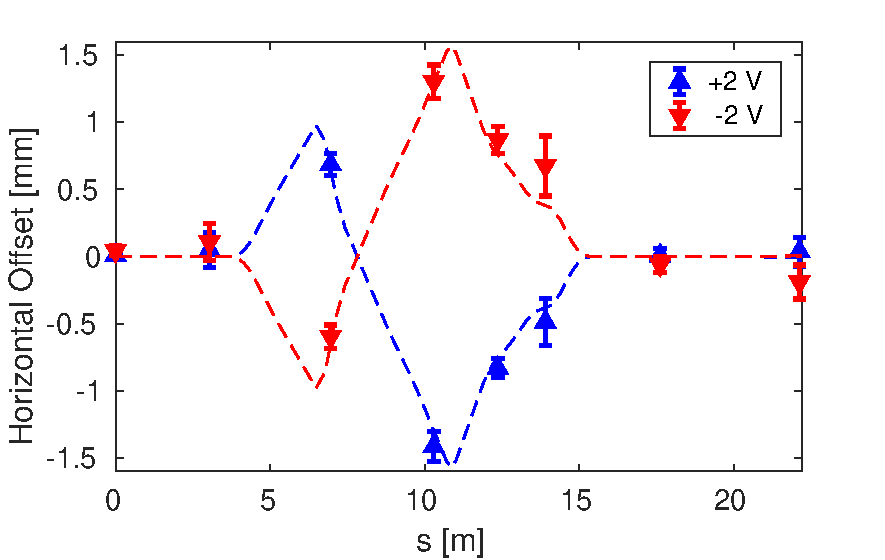
\includegraphics[width=\columnwidth]{figs/optics/orbClos}% Here is 
	%how to 
	%import EPS art
	\caption{\label{f:orbClos}
	}
\end{figure}

Fig.~\ref{f:orbClos} shows the orbit closure measured in the BPMs in and around 
the correction chicane. The BPM orbit is compared to the expected trajectory in 
the nominal optics for the chicane. The measurement and the model are in good 
agreement. A maximum horizontal offset of 1.5~mm inside the chicane is reduced 
to less than 0.1~mm after the chicane.

\subsection{\label{ss:timing}Correction Timing}

To be able to correct intra-pulse phase variations the arrival of the amplifier 
drive voltage at the kicker strips must be precisely synchronised with the 
arrival time of the beam. The correction timing is controlled by the 
feedforward controller and has been optimised with beam based measurements, as 
presented here.

\begin{figure}
	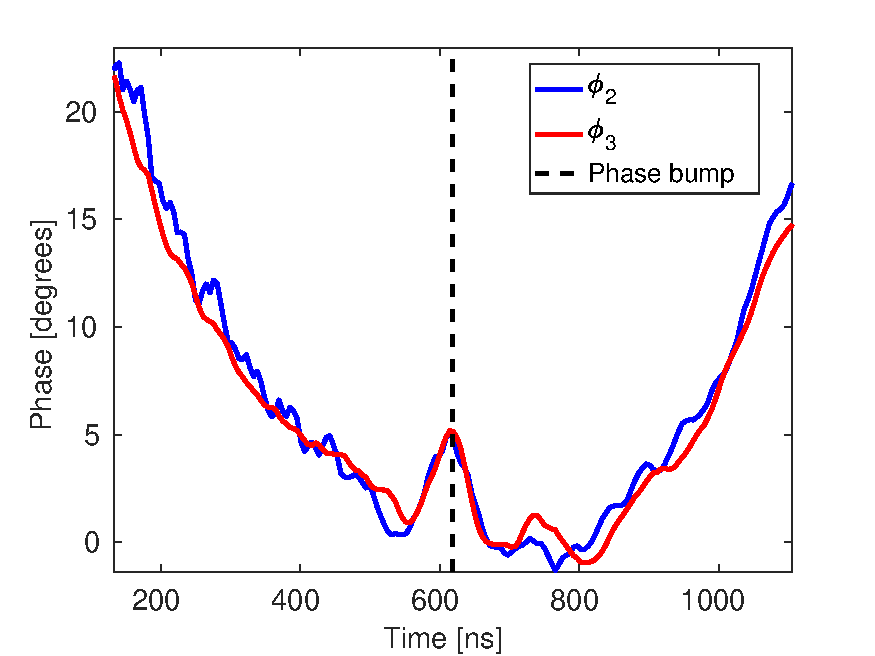
\includegraphics[width=\columnwidth]{figs/comis/bumpMon2Mon3}% Here is 
	%how to 
	%import EPS art
	\caption{\label{f:bumpMon2Mon3}
	}
\end{figure}

The waveforms of the klystrons were changed to produce a clear phase bump in 
the 
centre of the beam pulse. The bump is clearly visible in both \(\phi_1\) and 
\(\phi_3\), as shown in Fig.~\ref{f:bumpMon2Mon3}. This feature was used to 
determine the necessary delay in the controller output in order to align the 
PFF correction (the kicker voltage) with the beam. 

\begin{figure}
	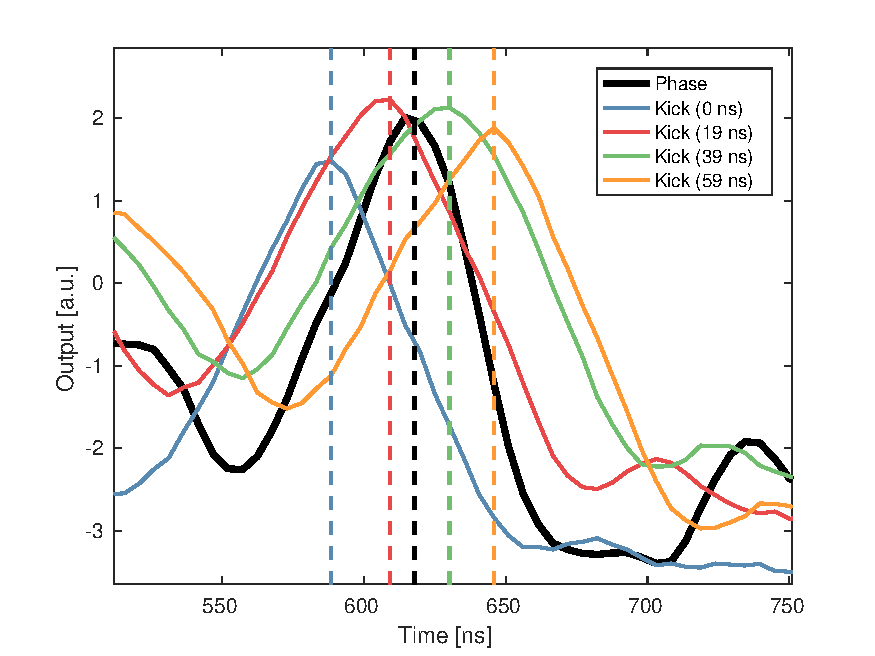
\includegraphics[width=\columnwidth]{figs/comis/absDelay_zoom}% Here is 
	%how to 
	%import EPS art
	\caption{\label{f:absDelay_zoom}
	}
\end{figure}

The PFF correction was applied in interleaved mode. The phase shift at 
\(\phi_3\) caused by the PFF system can then be calculated by taking the 
difference between the `PFF On' and `PFF Off' pulses in the dataset. For the 
optimal system setup this difference should be identical to the initial (`PFF 
Off') phase but with opposite sign.

Fig.~\ref{f:absDelay_zoom} shows the difference (labelled `kick') compared to 
the initial phase for four different controller output delays, zoomed in to the 
region of the pulse with the added phase bump. The differences are sign flipped 
and scaled to facilitate comparisons with the initial phase. Dashed lines 
indicate the time of the phase bump peak in each case. 

\begin{figure}
	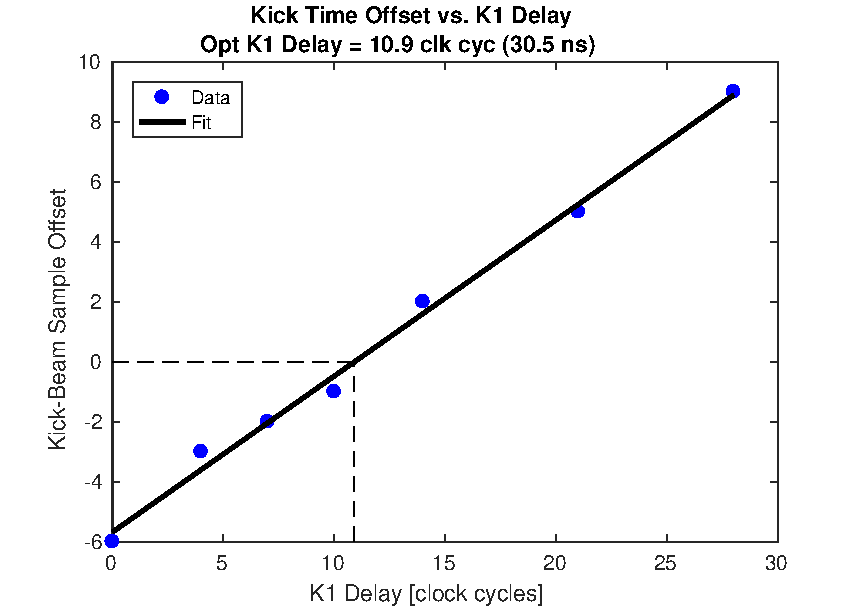
\includegraphics[width=\columnwidth]{figs/comis/OptDelayFit}% Here is 
	%how to 
	%import EPS art
	\caption{\label{f:OptDelayFit}
	}
\end{figure}

With the correction applied as soon as possible (`Kick 0 ns', blue) the phase 
bump in the applied kick arrives early, at 588~ns in the figure compared to 
618~ns for the initial phase. This proves the PFF system meets the latency 
requirements, with a total system latency of around 350~ns compared to the 
380~ns beam time of flight. As the output delay from the controller is 
increased, the phase bump in the applied kick overlaps and then trails its 
location in the initial phase. Fitting the difference in the peak positions vs. 
the output delay yields an optimal controller delay of \(31\pm4\)~ns 
(Fig.~\ref{f:OptDelayFit}).

\begin{figure}
	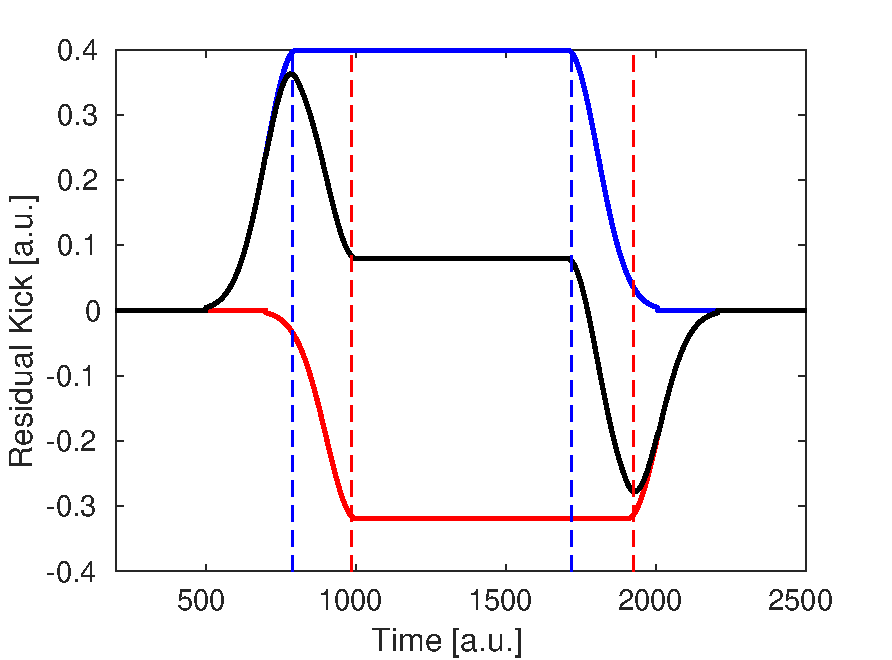
\includegraphics[width=\columnwidth]{figs/comis/relDelay_sim}% Here is 
	%how to 
	%import EPS art
	\caption{\label{f:relDelay_sim}
	}
\end{figure}

The previous measurement verifies the timing of the correction signal applied 
to the first kicker (\(\mathrm{K_1}\)), which provides the phase shift in the 
chicane. The second kicker (\(\mathrm{K_2}\)) ensures the beam orbit downstream 
of the chicane is unaffected by the PFF correction, but has a negligible effect 
on the beam phase. The beam time of flight between the kickers is about 36~ns, 
thus the PFF correction voltage must arrive at \(\mathrm{K_2}\) 36~ns later 
than the correction at \(\mathrm{K_1}\). If this is not the case the PFF system 
will cause horizontal position offsets downstream of the chicane.

\begin{figure}
	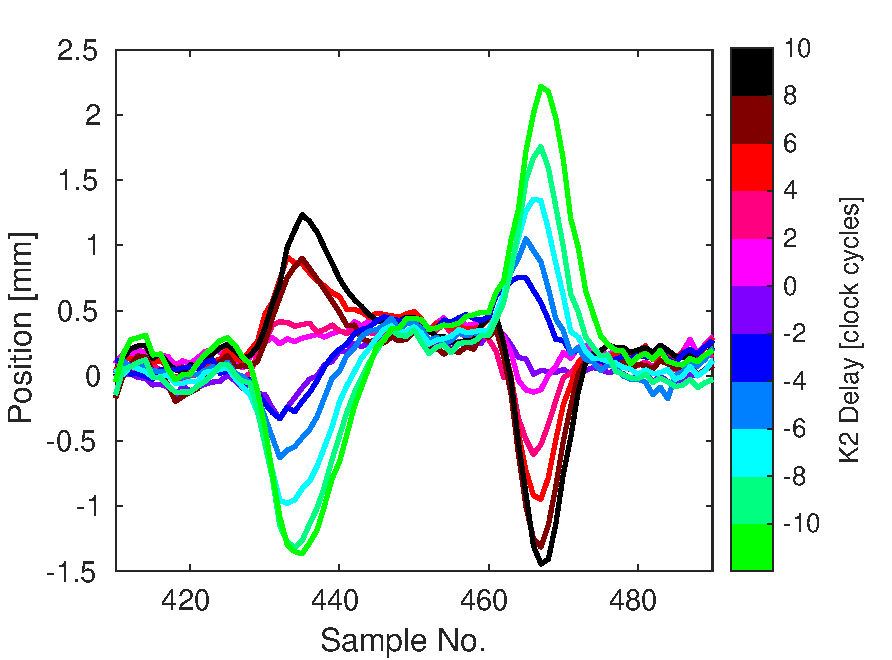
\includegraphics[width=\columnwidth]{figs/comis/relDelay_traces}% Here is 
	%how to 
	%import EPS art
	\caption{\label{f:relDelay_traces}
	}
\end{figure}

Fig.~\ref{f:relDelay_sim} illustrates the effect of the 
correction not being synchronised with the beam at 
both kickers. A constant voltage is applied to the kickers, as shown in red and 
blue. The total kick, the sum of the two, is in black and should be zero for 
the whole pulse duration in the ideal PFF setup. A time offset between the 
kicker voltages with respect to the beam leads to a large residual kick at the 
start and end of the pulse. If the kicker voltages have different magnitudes 
there is also a constant offset in the central portion of the pulse.

\begin{figure}
	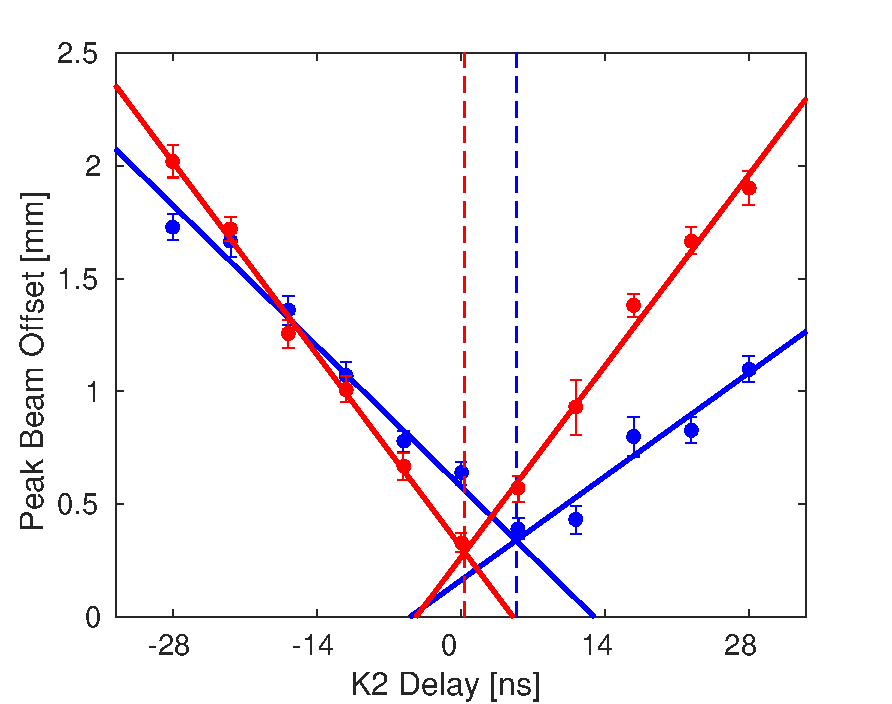
\includegraphics[width=\columnwidth]{figs/comis/relDelay_fit}% Here is 
	\caption{\label{f:relDelay_fit}
	}
\end{figure}

The amplifier-to-kicker cables for \(K_2\) are longer than the \(K_1\) cables 
to compensate for additional beam time of flight. The 
correction output delay for each kicker can also be fine-tuned independently on 
the feedforward controller. 

To verify the timing of the \(K_2\) correction output the feedforward 
controller was used to apply a constant kick to a 168~ns portion of the pulse. 
The kick was applied in interleaved mode, with the horizontal position 
difference between the PFF Off and PFF On pulses measured in a BPM downstream 
of the chicane.
Fig.~\ref{f:relDelay_traces} shows this difference for different delays 
applied to the \(K_2\) correction output with respect to the \(K_1\) output, 
ranging from -28~ns to +28~ns. The response is similar to the simulated example 
in Fig.~\ref{f:relDelay_sim}, as expected.

The optimal delay for the \(K_2\) correction output minimises the size of the 
peaks resulting from residual kicks, and this is fitted for the peaks at both 
the leading and trailing end of the pulse in Fig.~\ref{f:relDelay_fit}. The 
fitted value is \(1.4\pm1.7\)~ns. During operation of the PFF system the 
\(K_2\) output was typically delayed by 2.8~ns with respect to \(K_1\). This is 
the minimum non-zero delay that can be applied by the feedforward controller 
(equivalent to one time period of the 357~MHz ADC clock frequency).

\subsection{\label{ss:gain}Correction Gain}

%PRL
\begin{figure}
	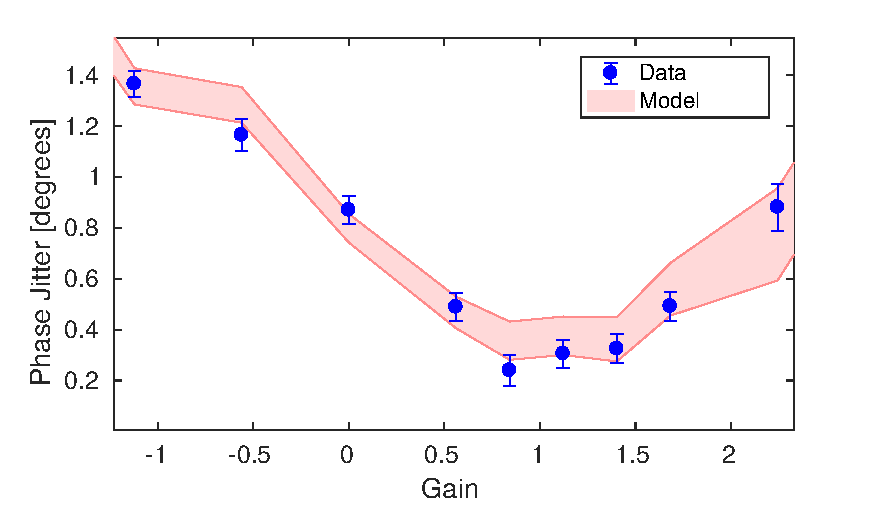
\includegraphics[width=\columnwidth]{figs/comis/gScan}% Here is 
	\caption{\label{f:gScan}
	}
\end{figure}

The PFF system acts to remove the \(\phi_1\) phase, multiplied by a `gain' 
factor, from the phase at \(\phi_3\). If the phases at \(\phi_3\) and 
\(\phi_1\) are fully correlated, and the jitters are identical, the optimal 
system gain is unity.
In practice the gain is chosen to achieve optimal 
performance for real beam conditions. A representative gain scan is shown 
in~Fig.~\ref{fig:gScan}. The optimal gain is typically in the range 
0.9--1.3. Also shown in Fig.~\ref{fig:gScan} is a prediction of 
the corrected phase jitter at \(\phi_3\), using a simple model including the 
initial beam phase jitters at \(\phi_1\) and 
\(\phi_3\), the upstream-downstream phase correlation, and the gain 
\cite{RobertsThesis}. The model reproduces the data.
%/PRL

\section{\label{s:results}Results}

\subsection{\label{ss:meanJit}Correction of Mean Phase Jitter}

%PRL
The effect of the PFF system on the pulse-to-pulse jitter, i.e. the jitter on 
the mean phase of each beam pulse, is shown in Fig~\ref{fig:meanJit} for a 
dataset of around ten minutes duration.
The pulse-to-pulse phase jitter is reduced from  \(0.92\pm0.04^\circ\) to 
\(0.20\pm0.01^\circ\), meeting CLIC-level phase stability. 
The system acts to remove all correlation between the upstream and 
downstream phase, reducing an initial correlation of \(96\pm2\%\) to 
\(0\pm7\%\) for this dataset.
Given the incoming upstream phase jitter and 
measured upstream-downstream correlation, the performance is consistent with 
the theoretically predicted correction of \(0.26\pm0.06^\circ\).
%/PRL

Best mean jitter

\begin{figure}
	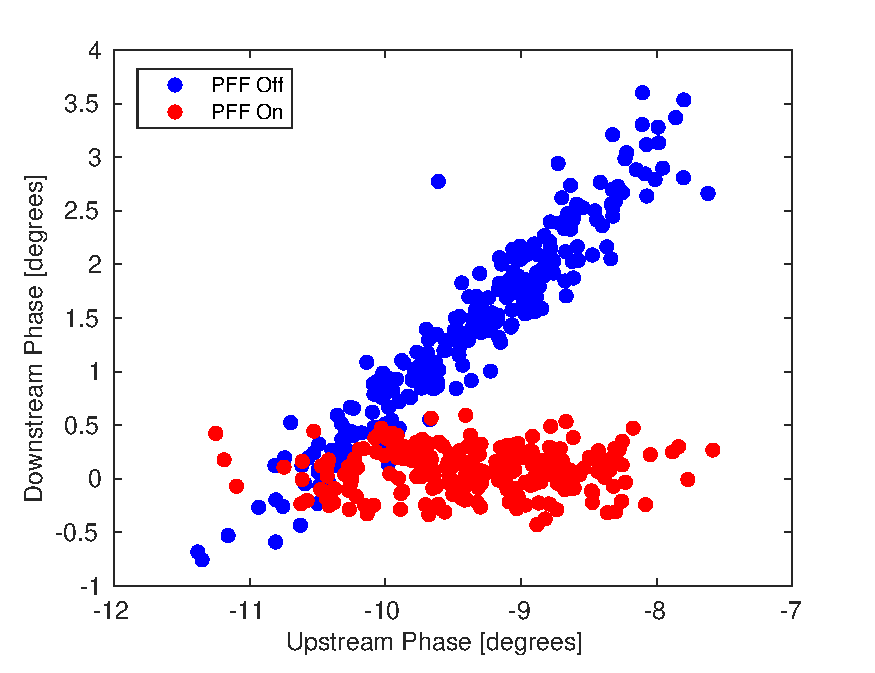
\includegraphics[width=\columnwidth]{figs/res/bestUpDownScatter}% Here is 
	\caption{\label{f:bestUpDownScatter}
	}
\end{figure}

\subsection{\label{ss:meanJit}Correction of Pulse Shape}
% PRL
The PFF system simultaneously corrects pulse-to-pulse phase jitter and phase 
variations within the 1.2~\(\mu s\) beam pulse at CTF3. 
Fig.~\ref{fig:shape} shows the effect of the PFF system on the intra-pulse 
phase variations. The PFF system was operated in interleaved mode, with 
the correction applied to alternating pulses only. This allows 
the initial (`PFF Off') and corrected (`PFF On') downstream phase at \(\phi_3\)
to be measured at the same time. The \(\phi_1\) (PFF input) phase 
is also shown for comparison. 

Approximately 440~ns portion of the pulse is 
within the \(\pm 6^\circ\) dynamic range of the PFF system, and can be 
corrected to zero nominal phase. 
This time duration for the full correction exceeds the CLIC drive-beam pulse 
length of 240ns and in any case the CLIC design avoids such 
a large phase sag~\cite{CLICCDR}. 
Vertical dashed lines in Fig.~\ref{fig:shape} mark the 440~ns portion of 
the pulse where full correction is possible.

Within the range the PFF system flattens the phase, and almost all variations 
are removed. 
Residual offsets are still present where there are small uncorrelated 
differences between the initial phase at \(\phi_1\) and \(\phi_3\). 
The average intra-pulse phase variation (rms) over the dataset is reduced from 
\(0.960\pm0.003^\circ\) (PFF off), to \(0.285\pm0.004^\circ\) (PFF on).
%/PRL

Best shape

\begin{figure}
	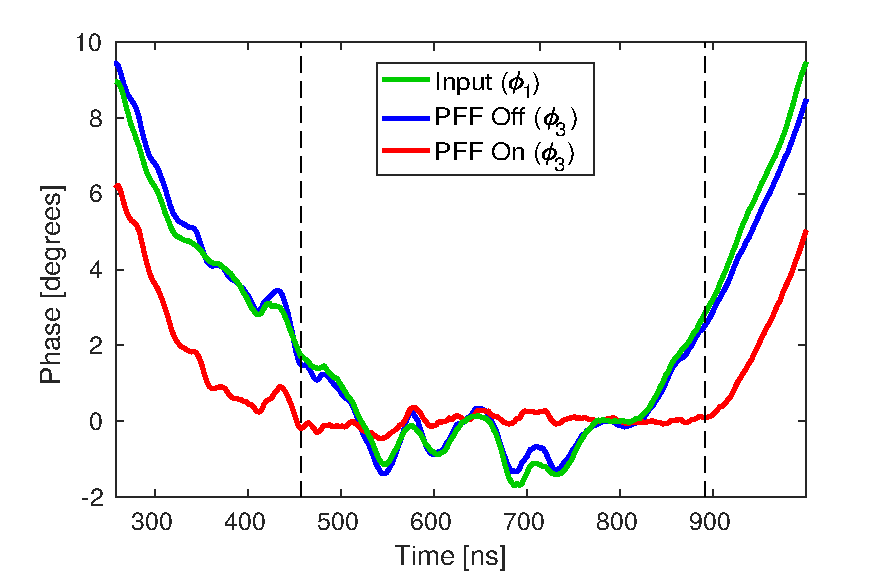
\includegraphics[width=\columnwidth]{figs/res/shape}% Here is 
	\caption{\label{f:shape}
	}
\end{figure}

\subsection{\label{ss:longResults}Long Term Results}

Long term correction and issues.

\begin{figure}
	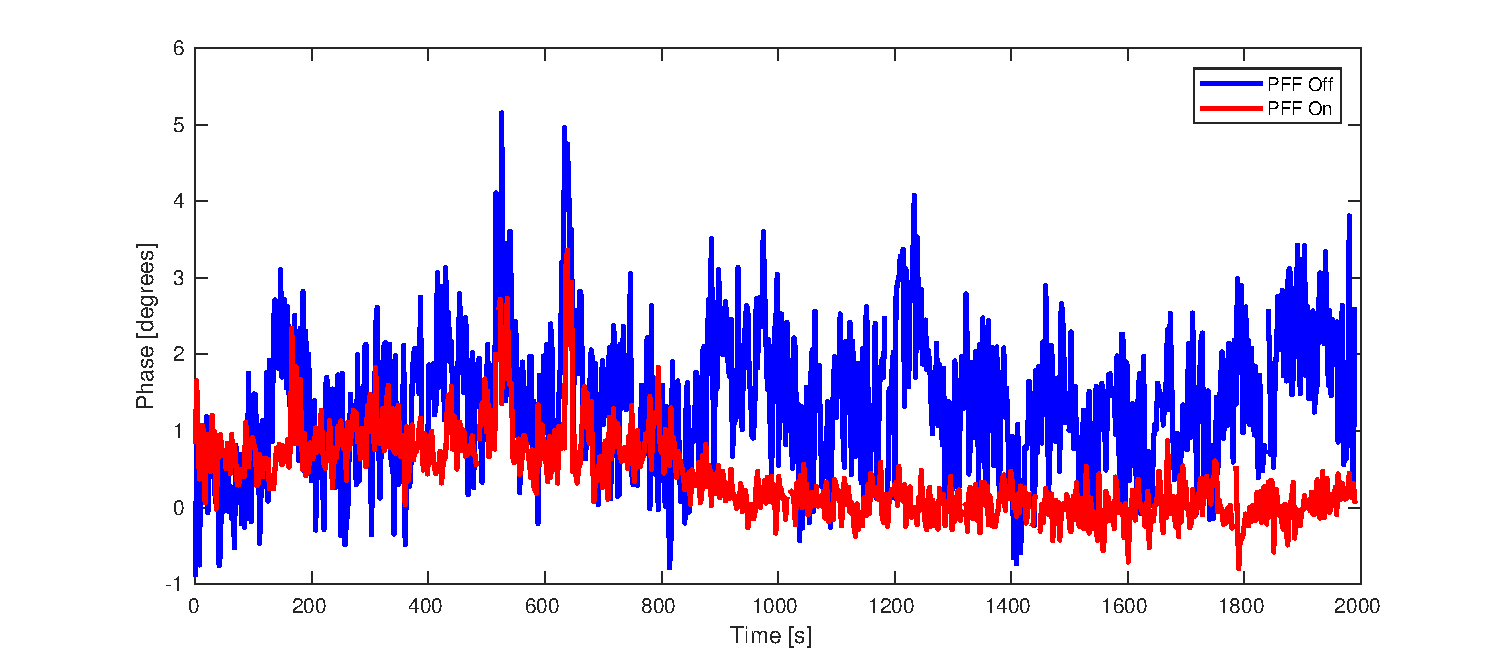
\includegraphics[width=\columnwidth]{figs/res/longMeanMon3}% Here is 
	\caption{\label{f:longMeanMon3}
	}
\end{figure}
\begin{figure}
	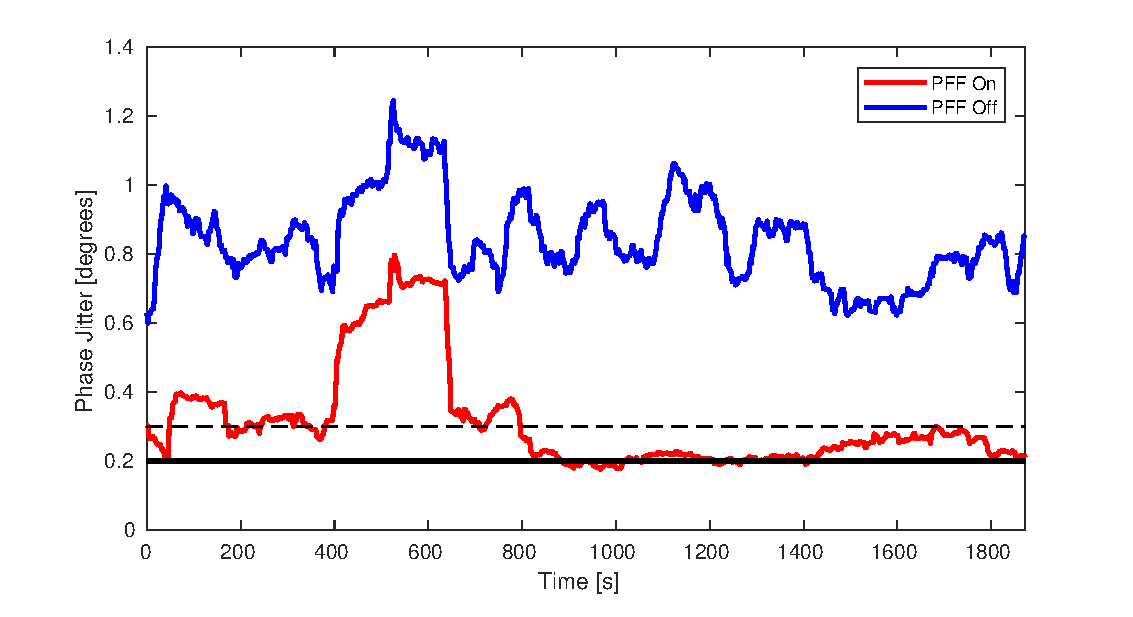
\includegraphics[width=\columnwidth]{figs/res/JitNext50}% Here is 
	\caption{\label{f:JitNext50}
	}
\end{figure}
\begin{figure}
	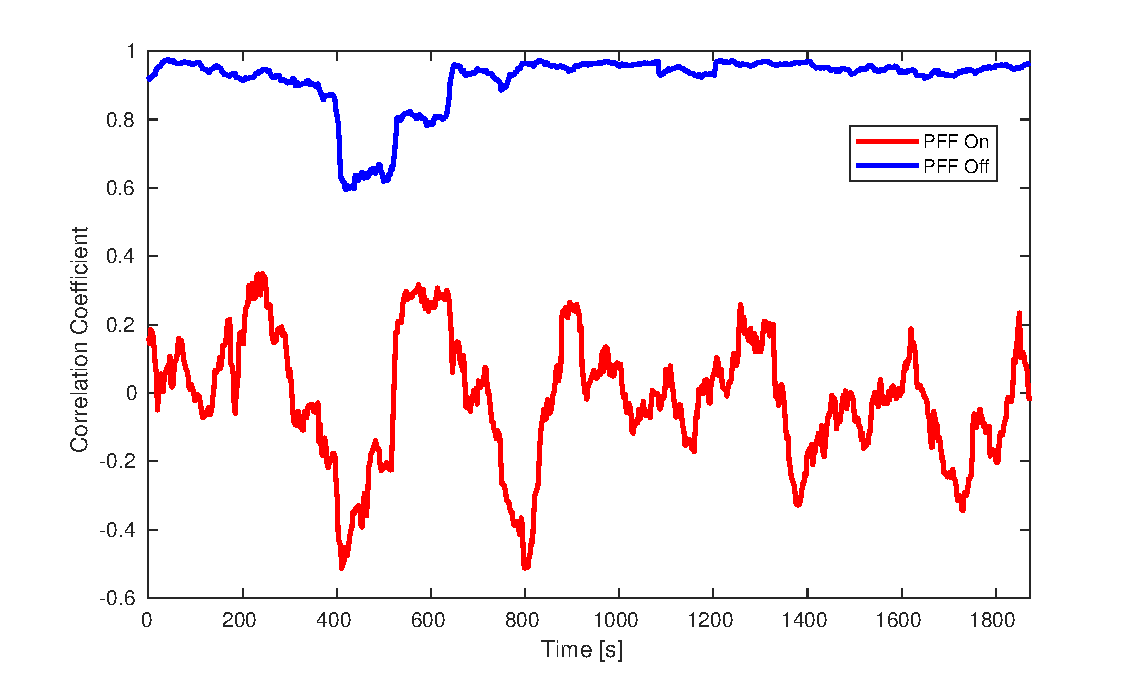
\includegraphics[width=\columnwidth]{figs/res/CorrNext50}% Here is 
	\caption{\label{f:CorrNext50}
	}
\end{figure}

\section{\label{s:conc}Conclusions}

\begin{acknowledgments}

\end{acknowledgments}

\bibliography{pff_prab}

\end{document}
